\documentclass{ieeeaccess}
\usepackage{cite}
\usepackage{amsmath,amssymb,amsfonts}
\usepackage{graphicx}
\usepackage{textcomp}
\usepackage{multirow}
\usepackage{mathtools}
\usepackage{subfigure}
\DeclarePairedDelimiter{\abs}{\lvert}{\rvert}
\def\BibTeX{{\rm B\kern-.05em{\sc i\kern-.025em b}\kern-.08em
T\kern-.1667em\lower.7ex\hbox{e}\kern-.125emX}}

\usepackage{algorithm}
\usepackage{colortbl}
\usepackage{algpseudocode}
\usepackage{tabularx}
\usepackage{arydshln}
% \usepackage[algcompatible]{algpseudocode}
\usepackage{array}
\newlength\savedwidth
\newcommand{\wcline}[1]{\noalign{\global\savedwidth\arrayrulewidth\global\arrayrulewidth 1.0pt} \cline{#1}
\noalign{\global\arrayrulewidth\savedwidth}}

\newcommand{\CCI}{\mathrm{CCI}} 
\newcommand{\HFDI}[1]{H_{image}(#1)}
\newcommand{\ti}{Android malware detection based on composition ratio of permission pairs}
\newcommand{\TI}{Android Malware Detection Based on Composition Ratio of Permission Pairs}
% \newcommand{\ti}{Android malware detection scheme using composition ratio of required permission pairs}
% \newcommand{\TI}{Android Malware Detection Scheme Using Composition Ratio of Required Permission Pairs}

\newcommand{\myfigurename}{Fig.}
\newcommand{\mytablename}{Table}
% Require$B$H(BEnsure$B$r(BInput$B$H(BOutput$B$K$9$k(B
\renewcommand{\algorithmicrequire}{\textbf{Input:}}
\renewcommand{\algorithmicensure}{\textbf{Output:}}
\newcommand{\etal}{\textit{et~al.}}


\begin{document}
\history{Date of publication xxxx 00, 0000, date of current version xxxx 00, 0000.}
\doi{10.1109/ACCESS.2017.DOI}

% \title{Android Malware Detection Scheme Based on Composition Ratio of Required Permission Pairs} 
% \title{Android Malware Detection Scheme \\Using Composition Ratio of Required Permission Pairs} 
\title{Android Malware Detection Based on Composition Ratio of Permission Pairs} 

\author{
  \uppercase{Hiroya Kato}\authorrefmark{1}, \IEEEmembership{Graduate Student Member, IEEE},
  \uppercase{Takahiro Sasaki}\authorrefmark{1},
  % \uppercase{Shuichiro Haruta\authorrefmark{1}, \IEEEmembership{Member, IEEE},
  and \uppercase{Iwao Sasase}.\authorrefmark{1}, \IEEEmembership{Senior Member, IEEE}}
\address[1]{Department of Information and Computer Science, Faculty of Science and Technology, Keio University 3-14-1 Hiyoshi, Kohoku, Yokohama, Kanagawa 223-8522, Japan}
% \tfootnote{This work is partly supported by the Grant in Aid for Scientific Research (No.17K06440) from Japan Society for Promotion of Science (JSPS).}

\markboth
{Kato \headeretal: \TI}
{Kato \headeretal: \TI}

\corresp{Corresponding author: Hiroya Kato (e-mail: kato@sasase.ics.keio.ac.jp).}

\begingroup
\newlength{\xfigwd}
\setlength{\xfigwd}{\textwidth}

\begin{abstract}
Detecting Android malware is imperative.
% Among various detection schemes, permission pair based ones are lightweight and effective, which causes .
Among various detection schemes, permission pair based ones are promising for practical detection.
% Permission pair based schemes are the most promising for practical application because most apps inevitably require permissions.
% Conventional schemes mainly rely on frequencies based scores and boolean vectors to detect malware.
However, conventional schemes cannot simultaneously meet requirements for practical use in terms of efficiency, intelligibility, and stability of detection performance.
% However, there remain serious problems for practical use in terms of efficiency, intelligibility, and stability of performance.
% In particular, even the latest scheme based on frequent pairs cannot satisfy the stability because of artifices by recent malware.
% Although the latest scheme depends on frequencies of permission pairs, it cannot satisfy the stability because of artifices by recent malware.
Although the latest scheme relies on differences of frequent pairs between benign apps and malware, it cannot meet the stability.
% because of artifices by recent malware.
% This is because recent malware tends to require not only necessary permissions but also unnecessary ones to imitate benign apps.
This is because recent malware tends to require unnecessary permissions to imitate benign apps, which makes using the frequencies ineffective.
% To meet all the requirements, in this paper, we propose \ti.  
% We focus on the fact that the ratio of a pair to all pairs in an app tends to be small in malware because of unnecessary permissions.
% We call this ratio Composition Ratio (CR).  
To meet all the requirements, in this paper, we propose Android malware detection based on a Composition Ratio (CR) of permission pairs.
We define the CR as a ratio of a permission pair to all pairs in an app.
We focus on the fact that the CR tends to be small in malware because of unnecessary permissions.
To obtain features without using the frequencies, we construct databases about the CR.
% For each class (benign apps and malware), four CR based databases are constructed from four aspects in terms of permissions, namely Android Permission (AP), Custom Permission (CP), Dangerous Permission (DP), and all permissions.
% In other words, the eight databases are prepared in total.  
For each app, we calculate similarity scores based on the databases.
% For each app, we calculate a similarity score for benign apps and one for malware on the basis of the databases.
% By doing this, even if malware requires unnecessary permissions, the effective features can be obtained from a new aspect.
Finally, eight scores are fed into machine learning (ML) based classifiers as features.
% By doing this, effective features can be obtained from a new aspect.
By doing this, stable performance can be achieved.
% The proposed scheme utilizes just eight-dimensional features, it can reduce training time and compatibility with other features, which means our scheme is efficient. 
Since our features are just eight-dimensional, the proposed scheme takes less training time and is compatible with other ML based schemes.
Furthermore, our features can quantitatively offer clear information that helps human to understand detection results.
Our scheme is suitable for practical use because all the requirements can be met.
% Our scores are easy to be understood because information about required permission pairs can be expressed as eight simple scores.
% Thus, since understandable information are provided for human, the proposed scheme also meets ``Intelligibility'', which is suitable for practical use.
By using real datasets, our results show that our scheme can detect malware with up to 97.3\% accuracy.
% convert information about permission pairs into just eight-dimensional features with maintaining comparable detection accuracy compared with a conventional scheme.
Besides, compared with an existing scheme, our scheme can reduce the feature dimensions by about 99\% with maintaining comparable accuracy on recent datasets.
% Besides, compared with a existing method, our scheme can reduce training time by about 91\% with maintaining comparable detection accuracy.
\end{abstract}

\begin{keywords} 
 Android malware detection, Permission pairs, Composition ratio, Practical detection 
 \end{keywords}

\titlepgskip=-15pt

\maketitle

\section{Introduction}  \label{sec:introduction}
Android is the most popular smartphone platform occupying 85\% of market share in the world \cite{idc}.
Smartphone is an essential tool for many people, and Android apps can provide various services such as online banking and games.
Because of its popularity, smartphones running on Android system have become the main target of attackers \cite{saracino2016madam}.
In the third quarter of 2019, approximately 365,000 new Android malware samples have been found \cite{wang2020review}.
Android malware is rapidly growing in an attempt to elaborately pretend benign apps.
Thus, using Android apps entails the risk of installing malware, which results in the urgency of devising practical detection schemes.

To detect sophisticated malware on the basis of various aspects, many detection methods have been proposed.
% Existing detection methods are roughly divided into two categories, namely ``network based methods'' \cite{wang2018detecting,garg2017network} and ``Android architecture based ones'' \cite{xu2016iccdetector,li2018significant, tao2017malpat, onwuzurike2019mamadroid}.  
Existing detection schemes are roughly divided into three categories, namely ``network traffic based schemes'' \cite{wang2018detecting,garg2017network} and ``inner interaction based ones'' \cite{aafer2013droidapiminer, deshotels2014droidlegacy, xu2016iccdetector, cai2018droidcat}, ``permission based ones'' \cite{sanz2013puma, li2018significant, liang2014permission, liu2014two, arora2019permpair}.
In network traffic based schemes \cite{wang2018detecting,garg2017network}, network traffic is used to create features for detecting malware.
These methods are helpful because most attackers are inclined to use network for achieving malicious purposes.  
However, network based methods are not applicable to malware that conducts attacks without networks.
Besides, they inevitably require running apps to collect features, which results in a certain runtime overhead.  
On the other hand, in inner interaction based schemes \cite{aafer2013droidapiminer, deshotels2014droidlegacy, xu2016iccdetector, cai2018droidcat}, features are extracted from various factors such as Application Programming Interface (API) calls and Inter-Component Communication (ICC) patterns.
These methods are instrumental in capturing detailed features of apps because there exists difference of the usage of the above factors between benign apps and malware. 
However, these types of schemes also suffer from runtime overhead to extract API calls and ICC patterns even if static analysis is adopted.
As features to realize lightweight and efficient detection, permission based schemes \cite{sanz2013puma, li2018significant, liang2014permission, liu2014two, arora2019permpair} are the most useful.
Thus, permission based schemes are the most promising for practical detection.
% Among various lightweight permission based schemes, we pay attention to permission pairs based schemes \cite{liang2014permission, liu2014two, arora2019permpair}.
Among various permission based schemes, ``permission pairs'' based schemes \cite{liang2014permission, liu2014two, arora2019permpair} are more effective and informative than a single permission based ones \cite{sanz2013puma, li2018significant}.
% Among permission usages, permission pairs are more informative than a single permission.
In other words, using permission pairs improves detection performance and helps users and security engineers to understand detection results in the practical situations because the permission pairs can provide more detailed information about how permissions are used together.
% Furthermore, in \cite{arora2019permpair}, it is reported that permission pairs based scheme is more effective than single permission based ones.
% Thus, permission pairs based schemes \cite{liang2014permission, liu2014two, arora2019permpair} are promising for practical use.
These facts motivate us to pay attention to permission pairs based schemes \cite{liang2014permission, liu2014two, arora2019permpair} as attractive ones.  
Although various permission pairs based schemes \cite{liang2014permission, liu2014two, arora2019permpair} have been proposed, none of them are able to simultaneously satisfy three critical requirements for practical use, which hinders the conventional schemes from being used practically.
To be specific, it is desirable that the following three requirements are satisfied.
\begin{enumerate}
  % \item Efficiency: reducing memory consumption for storing feature vectors and computational cost for detection system, which causes lightweight detection.
  % \item Efficiency: Detection system needs to achieve accurate detection by using low-dimensional feature vectors and compact informative data in order to realize lightweight detection and the feature fusion in machine learning.
  \item Efficiency: Practical detection systems need to realize accurate detection by using low-dimensional feature vectors and compact data, which achieves lightweight detection.  
    % Besides, the system must be compatible with other schemes to conduct the hybrid machine learning (ML) based detection with feature fusion.
    Compact features make systems compatible with other machine learning (ML) based schemes, which enables hybrid detection with feature fusion.
  \item Intelligibility: A practical scheme must offer clear information that helps human to understand detection results for justifying the results.
  % \item Tolerance: addressing recent malware that require unnecessary permissions to evade detection.
  \item Stability: A detection scheme must be able to detect both old and recent malware samples.
  % \item Detectability: achieving high detection performance.
\end{enumerate}
These requirements are very important to deploy detection schemes in practical situations.
However, none of the conventional permission pairs based schemes are able to simultaneously meet the three requirements.
In particular, we found that even the latest scheme \cite{arora2019permpair} cannot fulfill the stability because of artifices by recent malware whereas other requirements are met. 
This is because that scheme relies on the differences of frequencies of permission pairs between benign apps and malware samples.
Note that the frequency of a pair is normalized in a range of 0 to 1 in that scheme.
For example, when a pair appears in half of all the apps in a dataset, the frequency of the pair is expressed as 0.5.
Recent malware tends to require unnecessary permissions as well to imitate benign apps.
As a result, since more pairs appear in both benign apps and malware, the frequency based detection gets ineffective.
% As a result, in most pairs, since the frequencies in malware tend to be higher than those in benign apps, the frequency based scores get ineffective.
% This is because recent malware tends to require not only necessary permissions but also unnecessary ones to imitate benign apps.
Thus, this work aims to devise a practical scheme that meets the above requirements by using a new tendency.

% In order to fulfill the three requirements, in this paper, we propose \ti.
In order to fulfill the three requirements, in this paper, we propose Android malware detection based on a Composition Ratio (CR) of permission pairs.
% We focus on the fact that the ratio of a permission pair to all pairs tends to be small in malware samples compared with benign apps.  
The CR is defined as a ratio of a permission pair to all pairs in an app.
For example, suppose that an app requires five permissions in its manifest file.
In this case, since the number of permission pairs is 10, the CR of pairs in the app is $0.1 = \frac{1}{10}$.
We focus on the fact that the CR tends to be small in malware compared to benign apps.
% We focus on the fact that the ratio of a permission pair to all pairs in an app tends to be small in malware because of unnecessary permissions.
% We call this ratio Composition Ratio (CR) of permission pairs.
The reason why there exists the difference of the CR is that unnecessary permissions tend to be contained in manifest files of malware samples to imitate benign apps.
% The CR is a numerical value which means how permission pairs are required with other ones.
% For example, suppose that an app requires five permissions in its manifest file.
% In this case, since the number of permission pairs is 10, the CR is $0.1 = \frac{1}{10}$.
To obtain features without using the frequencies, we construct databases regarding the CR in training datasets.
% For each label (benign apps and malware), these databases are constructed by using the CR of pairs created from four types of permissions, namely Android Permission (AP), Custom Permission (CP), Dangerous Permission (DP), and all permissions.
% In other words, the eight databases are prepared in total.  
For each app, we calculate eight similarity scores on the basis of the databases.
% For each app, we calculate a similarity score for benign apps and one for malware on the basis of the databases.
By doing this, even if recent malware requires unnecessary permissions, the helpful features of them can be obtained from a new aspect.
Thus, the proposed scheme can satisfy ``Stability''.
Finally, our scores are used as features in ML for detection.
% The proposed scheme calculates eight scores on the basis of the CR based similarity.
Since the proposed scheme utilizes just eight-dimensional features, it can realize reducing computational cost of training and compatibility with other features, which results in satisfaction of ``Efficiency''.  
Besides, our scores can quantitatively offer clear information that what types of permission pairs dictate detection results.
% Our scores are easy to be understood because information about required permission pairs can be expressed as eight simple scores.
Thus, since numerical evidence is provided for human, the proposed scheme also meets ``Intelligibility''.
Since all the requirements can be met, our scheme is more suitable for practical use.

The contributions of this paper are as follows:
\begin{enumerate}
  \item We discovered the fact that permissions pairs in benign apps also tend to appear frequently in recent malware samples.
    This fact causes degradation in detection performance of the latest permission pairs based scheme.
  \item We propose a more practical malware detection scheme using the CR of permission pairs. 
    To the best of our knowledge, this work first proposes using the CR for malware detection.
  \item The proposed scheme enables to not only realize stable detection but also offer numerical evidence to human.
    % \item To the best of our knowledge, this paper is the first work that proposes a novel scheme for properly utilizing permission pairs to correctly distinguish benign apps from malware.
  \item Our scheme is compatible with other ML based schemes because our features are just eight-dimensional ones, which enables hybrid detection.
\end{enumerate}
% These contributions can provide a robust detection scheme against recent malware. 

The rest of this paper is constructed as follows. 
Related work is introduced in Section \ref{sec:related_work}.
Motivation of this work is described in Section \ref{sec:motivation}.
The shortcoming of conventional schemes are explained in Section \ref{sec:shortcoming}.
The proposed scheme is presented in Section \ref{sec:proposed_method}.
Evaluation results and discussion are shown in Section \ref{sec:simulation}.
Limitations of our scheme are described in Section \ref{sec:simulation}.
Finally, the conclusion of this paper and future work are presented in Section \ref{sec:conclusion}.

\section{Related Work} \label{sec:related_work}
Android malware detection schemes have been proposed on the basis of various aspects in order to detect sophisticated malware.
In this section, we introduce representative schemes.
Android malware detection methods are roughly divided into three categories, namely ``network traffic based methods'' \cite{wang2018detecting,garg2017network} and ``inner interaction based ones'' \cite{aafer2013droidapiminer, deshotels2014droidlegacy, xu2016iccdetector, cai2018droidcat}, ``permission based ones''  \cite{sanz2013puma, li2018significant, liang2014permission, liu2014two, arora2019permpair}.

\subsection{Network Traffic based Scheme}
In network traffic based schemes \cite{wang2018detecting,garg2017network}, network traffic is used to create features to detect malware.
In order to obtain solid evidence of malware, Wang \etal \cite{wang2018detecting} propose a method that pays attention to the occurrence of words regarding sensitive information in HTTP header of traffic data.
Malware uses HTTP-POST/GET schemes for sending sensitive information.
Therefore, semantic text features can be extracted from HTTP packets. 
The semantic text features mean the words such as ``latitude'', ``longitude'', and ``imei'', which is the unique identifier of a phone.
% Although that method can extract useful features including dynamic evidence, the malwares that encrypt malicious payloads cannot be efficiently detected.  
That scheme can effectively detect malware by using dynamic evidence because most attackers are inclined to use network for achieving malicious purposes.
However, recent malware cannot be efficiently detected by that scheme because they tend to encrypt malicious payloads.

To address encrypted traffic data, Garg \etal \cite{garg2017network} propose a scheme that leverages network traffic patterns in benign apps and malware.
The main idea of that scheme is that there exists the difference of network traffic patterns between benign apps and malware. 
That scheme is helpful because traffic patterns can be obtained even if malicious traffic is encrypted.
However, the method is not applicable to malware that conducts attacks without network.
% In addition to that, that method inevitably requires running apps to collect features, which results in a certain runtime overhead.
% Thus, features obtained by static analysis is desired for fast detection.
Thus, detection schemes that are able to deal with various types of malware samples are also needed.

\subsection{Inner interaction based scheme}
In inner interaction based schemes, features are extracted from factors such as API calls and ICC used in an app.

As an element that is useful in obtaining detailed features regardless of types of malware, API is very promising.
Aafer \etal \cite{aafer2013droidapiminer} propose a scheme using top-169 API calls which appear more frequently in malware than in benign apps to differentiate patterns of them.
As a similar scheme, Deshotels \etal \cite{deshotels2014droidlegacy} propose a scheme focusing on the fact that malware abuses sensitive API call.
In that scheme, malware samples are classified in accordance with malicious patterns predefined in advance. 
However, it is difficult for these schemes to detect the malware which carries out an attack by colluding with another malware because none of sensitive API calls are used by the main malware.
% Tao \etal \cite{tao2017malpat} propose a method that leverages permission-related APIs as features for ML.
% That method can achieve high detection performance with 50 highly sensitive APIs because it captures more detailed behaviors of apps by incorporating APIs with permissions.
% Although that method is useful, using the features based on APIs constantly requires retraining models whenever API specifications are changed.
% If new API calls are used in the latest benign apps and malware, the previous detection model that only utilizes old APIs for training might misjudge them.
% This retraining puts a burden on security engineers and, the delay of model updates results in missing rapidly growing malware.
% The retraining due to API update is mutual problem in API based methods \cite{deshotels2014droidlegacy, aafer2013droidapiminer,fan2017dapasa, tao2017malpat}.
% Thus, designing a method that is insusceptible to API updates is required.

To deal with sophisticated attacks such as a collusion attack, Xu \etal \cite{xu2016iccdetector} propose a scheme called ICCDetector focusing on the difference of ICC patterns between benign apps and malware.
ICC is inner communication among Android system and apps.
As a rule, ICC is mainly used for internal communication in a benign app.
Nevertheless, malware tends to communicate with other apps via ICC to carry out malicious actions.
% Although that method can effectively detect attacks including the collusion attack, it is difficult for that method to detect standard malware that conducts simple actions alone because of absence of ICC related features.
% In addition to this, that method uses 5,000 ICC-related features in total even after feature selection, which increases the computational cost of training. 
Thus, ICCDetector can effectively detect attacks including the collusion attack.
However, it is difficult for ICCDetector to deal with malicious behaviors that are conducted through obfuscation techniques called ``reflection'' because sensitive APIs are called via dynamic code constructs.

To cope with such clever techniques, Cai \etal \cite{cai2018droidcat} propose a scheme called DroidCat, which uses a diverse set of dynamic features based on ICC Intents.
DroidCat adopts a purely dynamic approach that resolves reflective calls at runtime.
Hence, that scheme is fully resilient against reflection.
However, DroidCat inevitably requires running apps to collect dynamic features, which results in a certain runtime overhead.  
Considering a huge amount of new malware is rapidly increasing, lightweight and efficient methods are desired.

\subsection{Permission based scheme}
As features to realize lightweight and efficient detection methods, permission based schemes are useful.
Sanz \etal \cite{sanz2013puma} propose a detection method using permissions extracted from apps.  
They noticed there exist several difference of required permissions in benign apps and malware.
% That method can differentiate benign apps from malware samples with an accuracy of about 86\%.
However, since that work just reveals that permissions are useful for detection, significant permissions were not inspected at all.
%$B$I$l$,=EMW$J%Q!<%_%C%7%g%s$J$N$+$J$I$O$"$-$i$+$K$7$F$$$J$+$C$?(B

To efficiently detect malware with fewer permissions, Li \etal \cite{li2018significant} propose a method that only utilizes significant permissions extracted from apps.
The idea of that method is that malware tends to require the common permissions that enable to conduct high risk operations such as accessing device information and personal information of users.
Instead of extracting and analyzing all permissions, that scheme conducts three levels of pruning by mining the permission data to identify the most significant permissions for detection.
% That method can detect malware in their datasets with just 22 permissions while maintaining over 90\% detection accuracy.
That scheme can maintain high detection accuracy with just 22 permissions.
% Therefore, it is desirable that researchers devise lightweight schemes to provide fast detection.
% $B$3$3$GLdBjE@$$$&$+$I$&$+(B
% However, none of the preceding schemes \cite{sanz2013puma, li2018significant} focuses on how to use the permissions to detect malware.
However, in \cite{sanz2013puma}, it is reported that the top five permissions in both the categories are exactly the same.
Thus, it is important to consider how such common permissions are used with other permissions in benign apps and malware.

Liang \etal \cite{liang2014permission} propose a rule based detection scheme by using permission combination.
The permission combination is useful to express the relationship between a permission and another.
They develop a tool that automatically generates rule sets based on frequencies of permission combinations to detect malware.
% That scheme can detect 83.57\% of the malware samples with a false positive rate of 12.47\% on their dataset when using a permission group of six.
That scheme can accurately detect malware samples when using a permission group of six.
However, utilizing permissions in a group of more than two can lead to a large number of patterns, and its expression will be complex.
Thus, detection with a group of more than two is not favorable for practical application because memory space consumption and computational cost will get high.

Similarly, Liu \etal \cite{liu2014two} propose a detection method using permission pairs.
The pairs are more useful than the combination of six permissions in terms of computational cost.
That scheme converts the requested permission pairs into a boolean vector because such a vector can represent information about pairs.
The boolean vector is fed into ML to detect malware.
Permission pairs are constructed only from top 40 permissions that are frequently used in benign apps and malware samples because utilizing all permission pairs considerably increase computational cost and memory consumption.
However, the boolean vector inevitably gets huge as considered permissions are increased in order to achieve high detection performance.
In other words, there exist a trade-off between detection accuracy and computational cost.
% Therefore, deciding the optimal number of permissions used for detection is required when that scheme is used for practical use.
Furthermore, in light of a practical use, the boolean vector is not sufficient to provide users with convincing information of analysis.
It is not easy for human to understand the meaning of a boolean vector whereas understandable information is important to justify detection results.
Thus, how to represent permission pairs for practical detection is one of the important goals.

% In order to identify the pairs of permissions that can be dangerous
% boolean $B$h$j%Z%"$r$&$^$/I=8=$7$?$_$?$$$J$3$H$r=q$-$?$$!#(B
To efficiently represent the permission pairs, Arora \etal \cite{arora2019permpair} propose a detection scheme called PermPair, which is based on frequencies of permission pairs in apps.
That scheme leverages the fact that frequencies of permission pairs appearing in malware samples are different from the ones in benign apps.
PermPair constructs databases on the basis of frequencies of permission pairs in prepared datasets of benign apps and malware.
The frequency of a pair is normalized in a range of 0 to 1.
In other words, when a pair appears in half of all the apps in a dataset, the frequency of the pair is expressed as 0.5.
By using the databases, PermPair calculates two similarity scores which represent how similar a characteristic of an app is to benign apps and malware samples in databases.
% When a pair exists in a database, the similarity score is calculated by simply summing up its normalized frequency.
When a pair exists in a database, its normalized frequency is simply added to the similarity score.
PermPair can convert permission pairs based information into just two scores, which results in providing clear information for human.
By comparing the two scores, PermPair can judge whether an app is malware or not and realize lightweight detection without ML.
% of malware samples in three datasets, namely Genome \cite{zhou2012dissecting},  Drebin \cite{arp2014drebin}, and Koodous~\cite{koodous}.
% Their result shows that PermPair is effective in detecting malware.
% with an accuracy of 95.44\%.

\section{Motivation of this work} \label{sec:motivation}
Although various schemes have been proposed, permission based schemes play an important role.
This is because permissions are essential factors to develop apps, and malware inevitably requires them to carry out malicious actions.
% Thus, permission is one of the integral features in Android malware detection.
Furthermore, permission based schemes \cite{sanz2013puma, li2018significant, liang2014permission, liu2014two, arora2019permpair} are lightweight compared with other detection schemes using features such as network traffic \cite{wang2018detecting,garg2017network}, API calls \cite{aafer2013droidapiminer, deshotels2014droidlegacy}, and ICC \cite{xu2016iccdetector, cai2018droidcat}.
In light of the predicament that a huge amount of malware is rapidly increasing, it is desirable that permission based detection schemes are practically used as a lightweight filter.
In particular, permission based detection is promising for a filter in the first step to identify malware.
Therefore, detecting more malware samples accurately by using permissions is very important to quickly deal with a huge amount of malware.
After permission based detection, other schemes should be applied to tested apps if needed.
% Therefore, it is necessary to make permission based schemes more practical.
% $B<BMQ2=$G$O$$$m$$$m$J$b$N$rAH$_9g$o$;$k$N$,NI$$$,!"(Bpermission$B$O7g$+$;$J$$$_$?$$$J$3$H=q$-$?$$!#(B
% For these reasons, we consider PermPair \cite{arora2019permpair} as the previous method, which is the latest detection.

Among permission based schemes, utilizing permission pairs are more informative than a single permission.
In other words, it is easier for users and security engineers to understand detection results because the permission pairs can represent how permissions are used together.
Furthermore, in \cite{arora2019permpair}, it is reported that permission pairs based scheme is more effective than single permission based ones as for detection accuracy.
% Thus, permission pairs based schemes \cite{liang2014permission, liu2014two, arora2019permpair} are promising for practical use.
These facts motivate us to pay attention to permission pairs based schemes \cite{liang2014permission, liu2014two, arora2019permpair} as conventional ones.
However, none of conventional schemes cannot simultaneously satisfy the three requirements, namely ``Efficiency'', ``Intelligibility'', and ``Stability'' explained in Section \ref{sec:introduction}.
In the subsequent section, we elaborate on the shortcomings.
% solve serious problems that hinder the schemes from being used practically.
Thus, this work aims to devise a more practical scheme that meets the above requirements.
% PermPair \cite{arora2019permpair}, which is one of the latest detection approaches motivate us to utilize permission pairs for detection.

% \section{Previous Method} \label{sec:previous_method}
% \subsection{Overview of Previous Method} 

\section{Shortcoming of Conventional Schemes} \label{sec:shortcoming}
\begin{table*}[h]
  \begin{center}
    \caption{Comparison of conventional permission pairs based schemes.}
    \label{tab:comparison_conv} 
    % \scalebox{0.9}{
    \begin{tabular}{c|c|c|ccc}
      % \hline
      \wcline{1-6} 
      \multirow{2}{*}{\rule{0pt}{2.3ex}\textbf{Reference}} & \multirow{2}{*}{\rule{0pt}{2.3ex}\textbf{Notation of Schemes}} & \multirow{2}{*}{\textbf{Mechanism}} &\multicolumn{3}{c}{\rule{0pt}{2.3ex}\textbf{Requirement}} \\ \cline{4-6}
                                                           &  & & \textbf{Efficiency} & \textbf{Intelligibility} & \textbf{Stability}\\ \hline
      % Li \etal (2018) \cite{li2018significant} & boolean vector of single permissions & Low & Low & High \\ 
      Liang \etal (2014) \cite{liang2014permission} & RSBS &  Frequency based rule set &  Low & High & Low \\ 
      Liu \etal (2014) \cite{liu2014two} & BVBS & boolean vectors  &  Low & Low & High \\ 
      Arora \etal (2019) \cite{arora2019permpair} & PermPair & Frequency based score &  High & High & Low \\
      \wcline{1-6}
      % \hline
    \end{tabular}
  % }
  \end{center}
\end{table*} 
\begin{figure*}[t]
  \centering
  \subfigure[Drebin (2010--2012)]{%
    \label{fig:permission_distribution_drebin}
    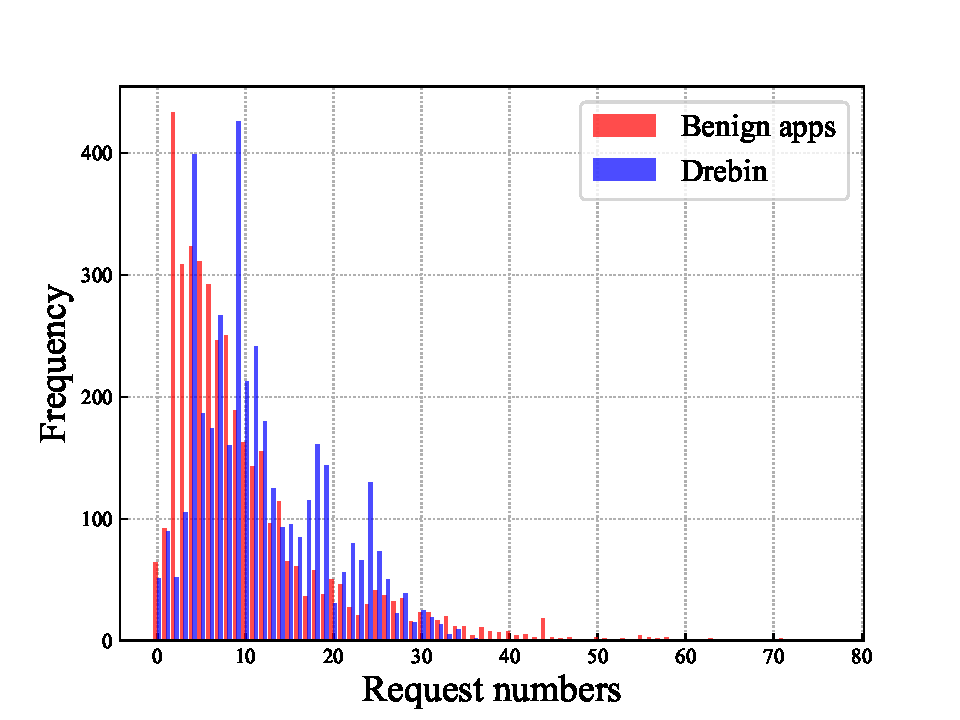
\includegraphics[scale=0.34]{./figures/Drebin_all_dist.pdf}
  } 
  \subfigure[Androzoo (2017--2020)]{ %
    \label{fig:permission_distribution_androzoo_new} 
    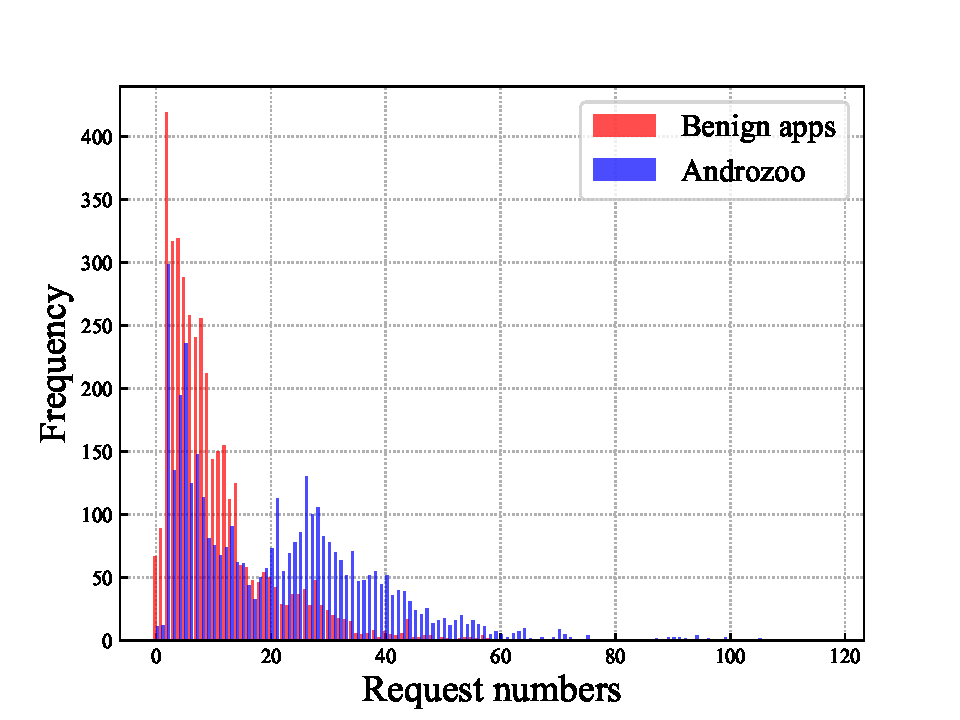
\includegraphics[scale=0.34]{./figures/Androzoo_all_dist_2017_2020.pdf}
  } 
  \subfigure[VirusShare (2018--2020)]{ %
    \label{fig:permission_distribution_virusshare} 
    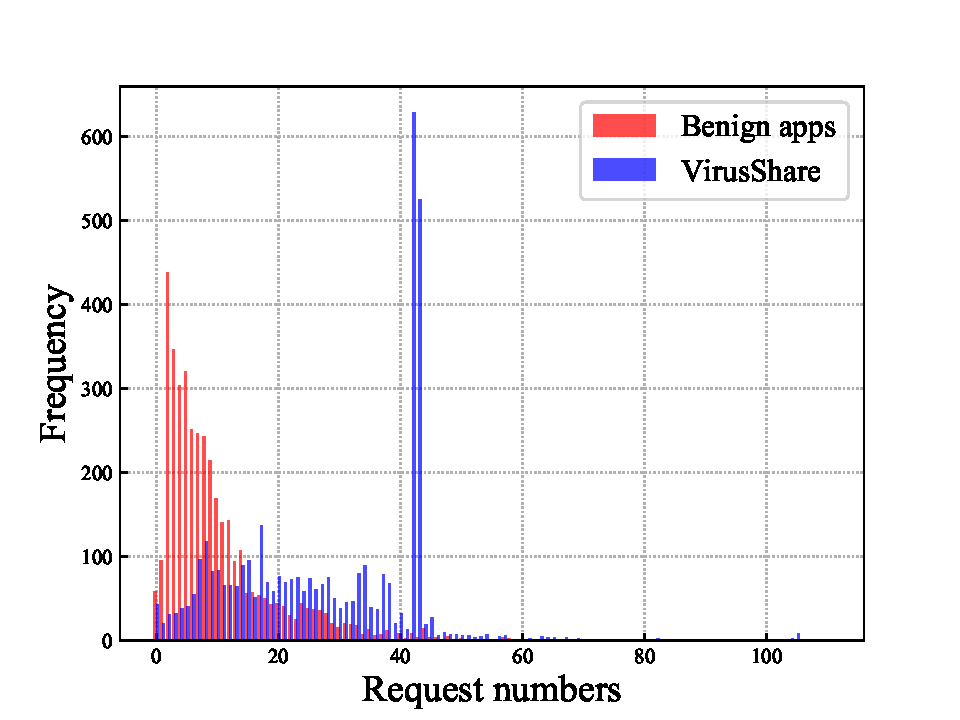
\includegraphics[scale=0.34]{./figures/VirusShare_all_dist.pdf}
  } 
  \caption{Distribution of the number of permissions required by benign apps and malware samples.}
  \label{fig:permission_distribution}
\end{figure*}
% Although various conventional permission pairs based schemes \cite{liang2014permission, liu2014two, arora2019permpair} have been proposed, none of them are able to simultaneously satisfy the three requirements, namely ``Efficiency'', ``Intelligibility'', and ``Stability'' explained in Section~\ref{sec:introduction}.  
To devise more practical schemes, detection systems must realize ``Efficiency'', ``Intelligibility'', and ``Stability''.
% \begin{enumerate}
  % % \item Efficiency: reducing memory consumption for storing feature vectors and computational cost for detection system, which causes lightweight detection.
  % \item Efficiency: achieving accurate detection by using low-dimensional feature vectors and compact informative data, which realizes lightweight detection and feature fusion in machine learning.
  % \item Intelligibility: offering understandable information about detection results to human, which achieves justification.
  % % \item Tolerance: addressing recent malware that require unnecessary permissions to evade detection.
  % \item Stability: yielding accurate detection performance against both old and recent malware.
  % % \item Detectability: achieving high detection performance.
% \end{enumerate}
These requirements are very important to deploy detection schemes in practical situations.
\mytablename~\ref{tab:comparison_conv} shows comparison of conventional permission pairs based schemes.
As shown in \mytablename~\ref{tab:comparison_conv}, there exist strong points and weak points in every scheme \cite{liang2014permission, liu2014two, arora2019permpair}.
Rule Set Based Scheme (RSBS) \cite{liang2014permission} and Boolean Vector Based Scheme (BVBS) \cite{liu2014two} only satisfy ``Intelligibility'' and ``Stability'', respectively.
On the other hand, although PermPair \cite{arora2019permpair} can meet ``Efficiency'' and ``Intelligibility'' by using the two simple scores, it cannot meet ``Stability''.
In the following subsections, we describe the above requirements in detail.

\subsubsection{Efficiency}
With regard to ``Efficiency'', RSBS \cite{liang2014permission} and BVBS \cite{liu2014two} have weak points.
In \cite{liang2014permission}, it is reported that RSBS cannot realize accurate classification with permission pairs unless it uses combinations of six permissions.
% In \cite{liang2014permission}, it is reported that RSBS cannot realize accurate classification with permission pairs whereas it can precisely classify apps into benign apps and malware by using combinations of six permissions.
Therefore, RSBS is not efficient because it needs to process numerous combinations of six permissions to create an effective rule set. 

In BVBS \cite{liu2014two}, boolean vectors tend to be large although such vectors can simply represent information about permission pairs.
For example, when 40 permissions are used for detection, ${}_{40}\mathrm{C}_2 = 780$ pairs are created, which means 780-dimensional sparse vectors.
Hence, such feature vectors are not efficient in terms of converting information about the pairs into features.
% , it is difficult to combine the high-dimensional features and other features based on different aspects.
These schemes need huge memory to store boolean vectors and combinations based rule set because the dimensions of the boolean vector and the number of rules inevitably get huge.  

Furthermore, most existing detection schemes adopt ML \cite{wang2018detecting, garg2017network, aafer2013droidapiminer, xu2016iccdetector, cai2018droidcat, sanz2013puma, li2018significant, liu2014two}, because it can yield high detection accuracy.
In every ML based scheme, various features have been defined.
The various features can be used together for enhancing detection performance, which results in inevitably increasing required space, training time, and complexity of model.
% In \cite{liu2014two}, high-dimensional vectors induce high computational cost to conduct training of machine learning. 
In light of the fact that huge training apps and regularly updating training data are required for high detection performance, it is desirable that dimensions of features are low to reduce the computational cost and complexity.
This is why converting information about permission pairs into low-dimensional features is important.
Since low-dimensional features can also provide compatibility with other schemes, for the purpose of realizing hybrid detection systems in the real world, this requirement must be satisfied.

\subsubsection{Intelligibility}
As for ``Intelligibility'', BVBS \cite{liu2014two} has a drawback.
Boolean vectors are not informative enough to describe the reason why an app is judged as malware, and vice versa.
This problem was also suggested in the other existing work \cite{wang2014exploring}.
On the other hand, RSBS \cite{liang2014permission} and PermPair \cite{arora2019permpair} can offer understandable information about detection results because rule set and scores can be utilized for interpretation.
In the practical use, clear information should be provided for users to understand detection results without adequate expertise.
Besides, security engineers need to understand detection results so that detailed analysis can be carried out.
Since the intelligibility can bring reliability of detection, this requirement must be met.

\subsubsection{Stability}
\definecolor{Gray}{gray}{0.85}  % Color Definition
In malware detection, ``Stability'' is the most important requirement.
In terms of ``Stability'', the RSBS \cite{liang2014permission} and PermPair \cite{arora2019permpair} have weak points.
In \cite{liang2014permission}, it is reported that frequency based rule set created from permission pairs cannot accurately distinguish benign apps from malware.
According to results in \cite{liang2014permission}, more than 55\% of benign apps are misjudged as malware whereas 99\% of malware samples are detected.
On the other hand, we found that PermPair \cite{arora2019permpair} is also incapable to detect recent malware samples because it can be invalidated by the recent tendency of required permissions.
To be specific, recent malware samples tend to require unnecessary permissions to imitate benign apps.

In order to confirm the tendency, we investigated the number of permissions required by benign apps and malware samples.
% \begin{figure*}[t]
  % \centering
	% % \makebox[0pt]{
    % \begin{tabular}{cc}
    % \subfigure[Androzoo (2011--2014)]{ %
      % \label{fig:permission_distribution_androzoo_old} 
      % 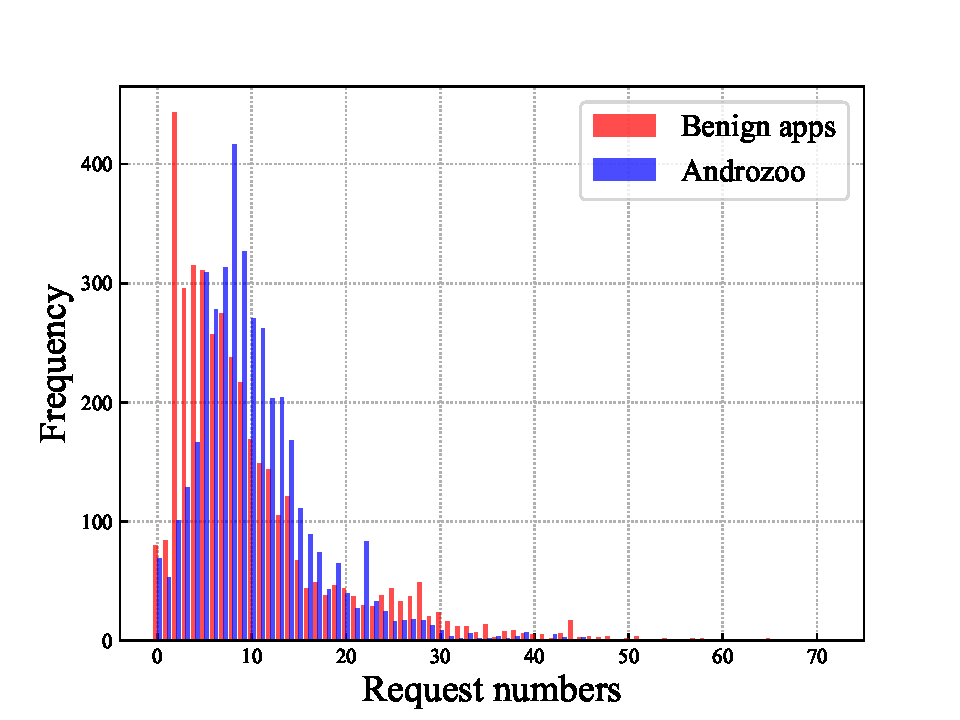
\includegraphics[scale=0.4]{./figures/Androzoo_all_dist_2011_2014.pdf}
    % }  & 
    % \subfigure[Drebin (2010--2012)]{%
      % \label{fig:permission_distribution_drebin}
      % 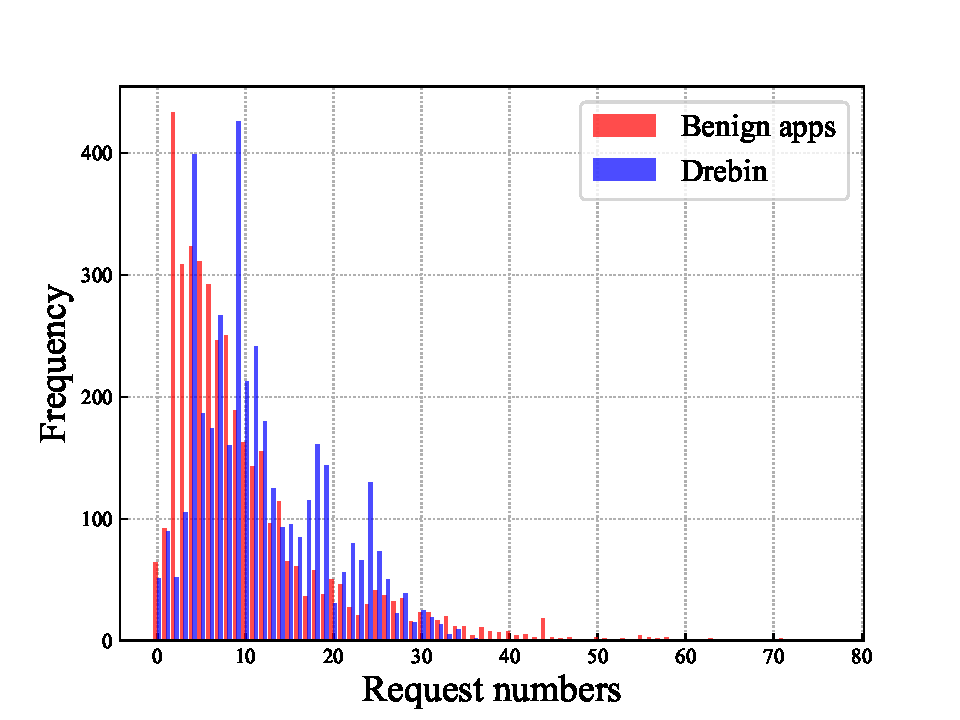
\includegraphics[scale=0.4]{./figures/Drebin_all_dist.pdf}
    % } \\
    % \subfigure[Androzoo (2017--2020)]{ %
      % \label{fig:permission_distribution_androzoo_new} 
      % 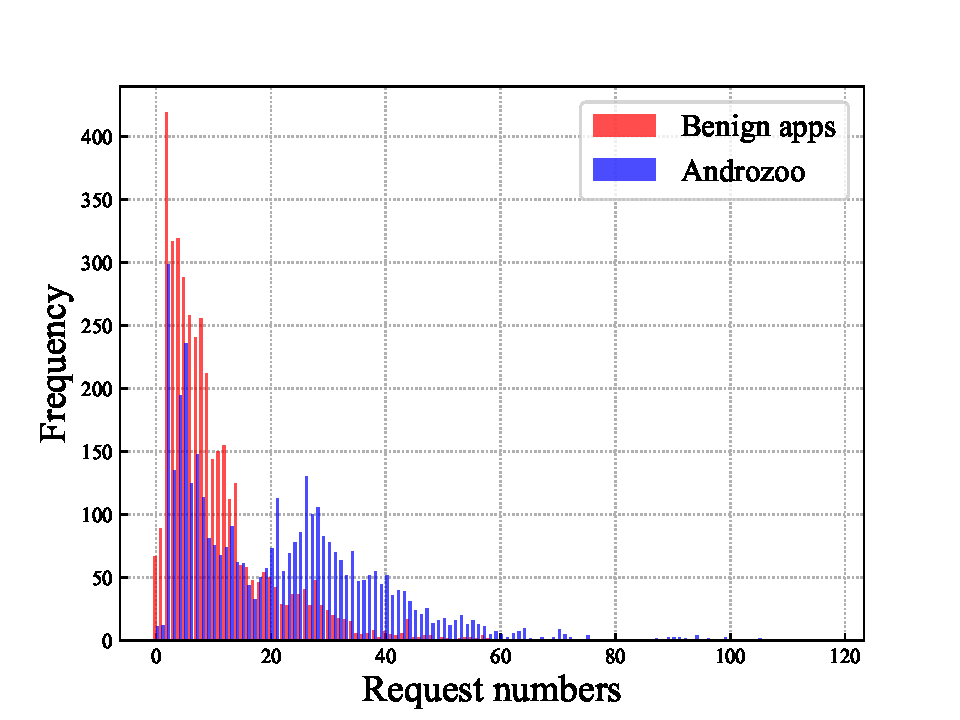
\includegraphics[scale=0.4]{./figures/Androzoo_all_dist_2017_2020.pdf}
    % } &
    % \subfigure[VirusShare (2018--2020)]{ %
      % \label{fig:permission_distribution_virusshare} 
      % 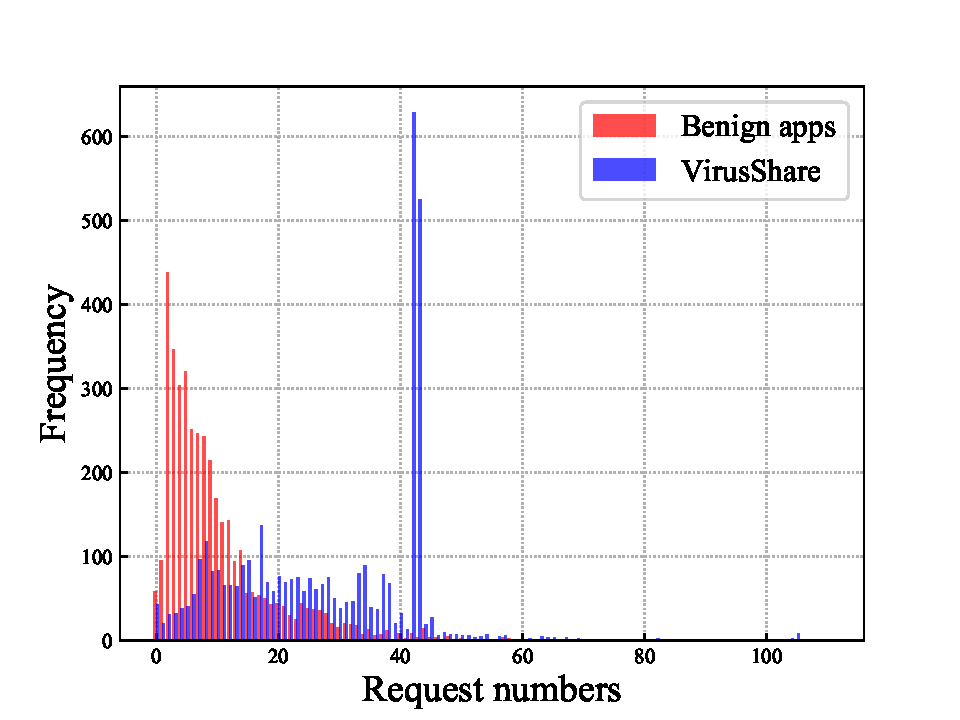
\includegraphics[scale=0.4]{./figures/VirusShare_all_dist.pdf}
    % } \\
  % % }
  % \end{tabular}
  % \caption{Distribution of the number of permissions required by benign apps and malware samples.}
  % \label{fig:permission_distribution}
% \end{figure*}
\myfigurename~\ref{fig:permission_distribution} shows distribution of the number of permissions required by benign apps and malware samples.
In \myfigurename~\ref{fig:permission_distribution_drebin}, 4,000 old malware samples are randomly selected from Drebin \cite{arp2014drebin} (2010--2012).
Meanwhile, in \myfigurename~\ref{fig:permission_distribution_androzoo_new} and \myfigurename~\ref{fig:permission_distribution_virusshare}, 4,000 recent apps are randomly selected from Androzoo \cite{allix2016androzoo} (2017--2020) and VirusShare \cite{virusshare} (2018--2020), respectively.
Furthermore, 4,000 benign apps are also randomly selected from Androzoo (2017--2020) for every figure in \myfigurename~\ref{fig:permission_distribution_drebin}, \myfigurename~\ref{fig:permission_distribution_androzoo_new}, and \myfigurename~\ref{fig:permission_distribution_virusshare}.
As shown in \myfigurename~\ref{fig:permission_distribution_drebin}, the distribution of malware is relatively similar to that of benign apps.  
In particular, most apps require less than 30 permissions. 
On the other hand, as shown in \myfigurename~\ref{fig:permission_distribution_androzoo_new} and \myfigurename~\ref{fig:permission_distribution_virusshare}, the distribution of malware is widely spread compared with \myfigurename~\ref{fig:permission_distribution_drebin}, which is old dataset.
In particular, many malware samples tend to require more than 30 permissions.
These investigation results demonstrate that recent malware samples tend to require unnecessary permissions compared with old ones.
% In \cite{sanz2013puma}, it is reported that the top five permissions in both the categories are exactly the same.
% Furthermore, through our experiments on our datasets, we discovered that top five permission pairs in benign apps also tend to be required by recent malware.
In addition, we also investigated top ten permission pairs in our datasets.
After that, we discovered that top ten permission pairs in benign apps also tend to be required by recent malware because of these tendencies, which causes degradation in detection performance of PermPair.  
\begin{table*}[t]
  \begin{center}
    \caption{Top ten permission pairs and their frequencies in Drebin, Androzoo, VirusShare, and the benign dataset. The pairs in gray cells are common ones.}
    \label{tab:top_pairs}
    % \scalebox{0.8}{
    \begin{tabular}{|c|c|c|c|c|c|c|c|} \hline
      \multicolumn{2}{|c|}{Drebin (2010--2012)} &\multicolumn{2}{c|}{Androzoo (2017--2020)} &\multicolumn{2}{c|}{VirusShare (2018--2020)}&\multicolumn{2}{c|}{Benign apps} \\ \hline 
      Permission pairs & Frequency & Permission pairs & Frequency & Permission pairs & Frequency & Permission pairs & Frequency \\ \hline
      INT:RPS & 0.908 & \multicolumn{1}{>{\columncolor{Gray}}c|}{\textbf{ANS:INT}} & 0.957 & \multicolumn{1}{>{\columncolor{Gray}}c|}{\textbf{ANS:INT}} & 0.981 & \multicolumn{1}{>{\columncolor{Gray}}c|}{\textbf{ANS:INT}} & 0.952\\ \hline
      \multicolumn{1}{|>{\columncolor{Gray}}c|}{\textbf{ANS:INT}} & 0.697 & INT:RPS & 0.850 & \multicolumn{1}{>{\columncolor{Gray}}c|}{\textbf{INT:WES}} & 0.969 & \multicolumn{1}{>{\columncolor{Gray}}c|}{\textbf{INT:WES}} & 0.668\\ \hline
      \multicolumn{1}{|>{\columncolor{Gray}}c|}{\textbf{INT:WES}}& 0.681 & ANS:RPS & 0.830 & \multicolumn{1}{>{\columncolor{Gray}}c|}{\textbf{ANS:WES}} & 0.961 & \multicolumn{1}{>{\columncolor{Gray}}c|}{\textbf{ANS:WES}} & 0.644\\ \hline
      ANS:RPS & 0.670 & \multicolumn{1}{>{\columncolor{Gray}}c|}{\textbf{INT:WES}} & 0.828 & \multicolumn{1}{>{\columncolor{Gray}}c|}{\textbf{AWS:INT}} & 0.941 & INT:WL & 0.530\\ \hline
      RPS:WES& 0.666 & \multicolumn{1}{>{\columncolor{Gray}}c|}{\textbf{ANS:WES}} & 0.810  & INT:RPS & 0.941 & ANS:WL & 0.521\\ \hline
      \multicolumn{1}{|>{\columncolor{Gray}}c|}{\textbf{ANS:WES}} & 0.525 & RPS:WES & 0.774 & \multicolumn{1}{>{\columncolor{Gray}}c|}{\textbf{ANS:AWS}} & 0.940 & \multicolumn{1}{>{\columncolor{Gray}}c|}{\textbf{AWS:INT}} & 0.495 \\ \hline
      INT:SSMS& 0.510 & \multicolumn{1}{>{\columncolor{Gray}}c|}{\textbf{AWS:INT}} & 0.666 & ANS:RPS & 0.936 & \multicolumn{1}{>{\columncolor{Gray}}c|}{\textbf{ANS:AWS}} & 0.493 \\ \hline
      INT:RBC& 0.502 & \multicolumn{1}{>{\columncolor{Gray}}c|}{\textbf{ANS:AWS}} & 0.663 & RPS:WES & 0.935 & WL:WES & 0.421\\ \hline
      RPS:RBC& 0.491 & AWS:RPS & 0.632 & \multicolumn{1}{>{\columncolor{Gray}}c|}{\textbf{AWS:WES}} & 0.934 & \multicolumn{1}{>{\columncolor{Gray}}c|}{\textbf{AWS:WES}} & 0.403\\ \hline
      RPS:SSMS& 0.479 & \multicolumn{1}{>{\columncolor{Gray}}c|}{\textbf{AWS:WES}} & 0.623 & AWS:RPS & 0.917 & INT:VR & 0.371\\ \hline
    \end{tabular}
    % }
  \end{center}
\end{table*} 
\begin{table}[t]
  \begin{center}
    \caption{The notation used for top permission pairs analysis.}
    \label{tab:notation_permission}
    \begin{tabular}{|c|c|} 
      \hline
      \textbf{Permission} & \textbf{Notation} \\ \hline 
       ACCESS\_NETWORK\_STATE & ANS \\ \hline 
       ACCESS\_WIFI\_STATE & AWS \\ \hline
       INTERNET & INT \\ \hline
       READ\_PHONE\_STATE & RPS \\ \hline
       RECEIVE\_BOOT\_COMPLETED & RBC \\ \hline
       SEND\_SMS & SSMS \\ \hline
       VIBRATE & VR \\ \hline
       WAKE\_LOCK & WL \\ \hline
       WRITE\_EXTERNAL\_STORAGE & WES \\ 
       \hline
    \end{tabular}
  \end{center}
\end{table}
\mytablename~\ref{tab:top_pairs} shows top ten permission pairs and their frequencies in Drebin, Androzoo, VirusShare, and the benign dataset.
Furthermore, \mytablename~\ref{tab:notation_permission} shows the notation used for top permission pairs investigation.
As shown in \mytablename~\ref{tab:top_pairs}, out of ten permission pairs, there exist three common pairs, namely ANS:INT, INT:WES, and ANS:WES between the Drebin (2010--2012) and Benign apps.
In other words, the permission pairs required by old malware in Drebin tend to be different from the ones of benign apps.
On the other hand, six permission pairs are common among benign apps, Androzoo (2017--2020), and VirusShare (2018--2020).
Moreover, their frequencies in Androzoo and VirusShare are higher than the ones in benign apps.
For example, ANS:INT is the most frequently required pairs in benign apps, and its frequency is 0.952.
Meanwhile, the frequencies are 0.957 and 0.981 in Androzoo and VirusShare, respectively.
Similarly, as for five other pairs, their frequencies in Androzoo and VirusShare are also high compared with benign apps.
In other words, it is natural that recent malware samples have permission pairs frequently required by benign apps, which means that more pairs appear in both benign apps and malware. 
As a result, apps cannot be correctly classified even through the frequencies are used.
% As a result, the frequencies of pairs in malware tend to be higher than those in benign apps.  
This is why we argue that detection schemes should not utilize the frequencies of permission pairs anymore.  
% Since the conventional schemes \cite{liang2014permission, arora2019permpair} are purely dependent on frequencies of permission pairs, their detection performance for recent malware can be degraded.
In particular, we discovered that PermPair \cite{arora2019permpair}, which is the latest scheme is considerably subject to this tendencies.
PermPair regards permission pairs with high frequencies as important ones.
% This is why malicious similarity score tend to be higher than benign one when a pair exists in both benign and malware database.
Frequency based databases in PermPair can be contaminated when recent malware samples are utilized to create them.
As a result, in most pairs, since the frequencies in malware tend to be higher than those in benign apps, the frequency based scores get ineffective.
Although PermPair can meet ``Efficiency'' and ``Intelligibility'', PermPair cannot deal with recent malware.

% one-hot coding to vectorize the extracted features
% Since conventional permission based schemes \cite{sanz2013puma, liang2014permission, li2018significant, arora2019permpair} mainly adopt features that are purely dependent on frequencies of permissions, malware samples can be misjudged as benign apps, and vice versa.
Therefore, to adopt permission pairs based detection for practical use, we must devise a novel scheme that satisfies the three above requirements simultaneously.

\section{Proposed Scheme} \label{sec:proposed_method}
\begin{figure*}[t]
  \centering
	% \makebox[0pt]{
    \begin{tabular}{cc}
    \subfigure[All permissions]{ %
      \label{fig:boxplot_all} 
      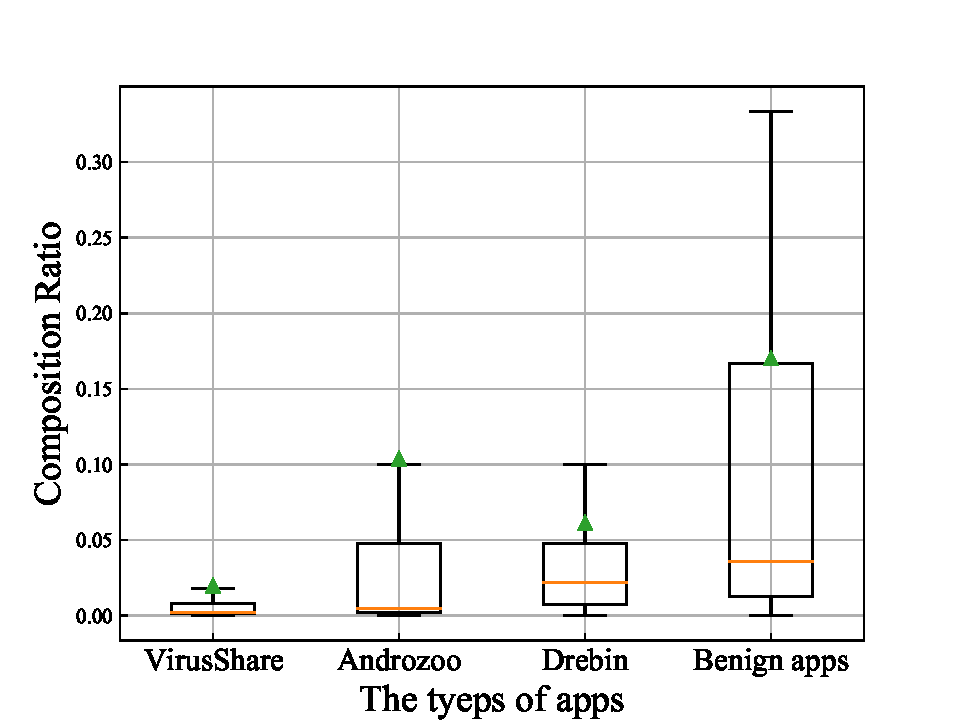
\includegraphics[scale=0.4]{./figures/com_ratio_all_box.pdf}
    }  & 
    \subfigure[Android permissions]{%
      \label{fig:boxplot_android}
      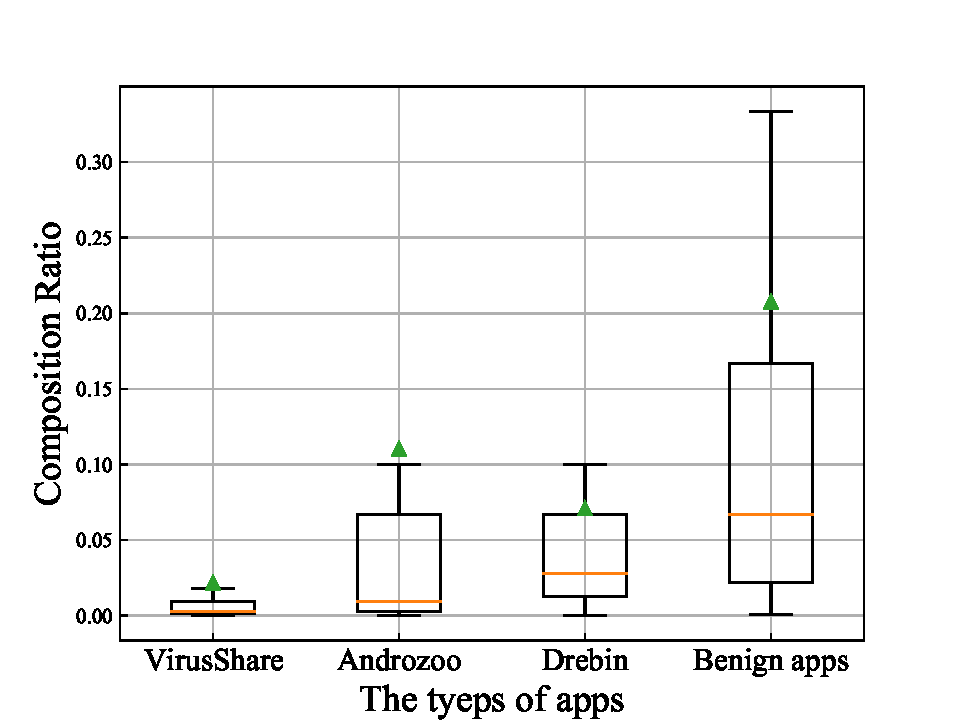
\includegraphics[scale=0.4]{./figures/com_ratio_android_box.pdf}
    } \\
    \subfigure[Dangerous permissions]{ %
      \label{fig:boxplot_dangerous} 
      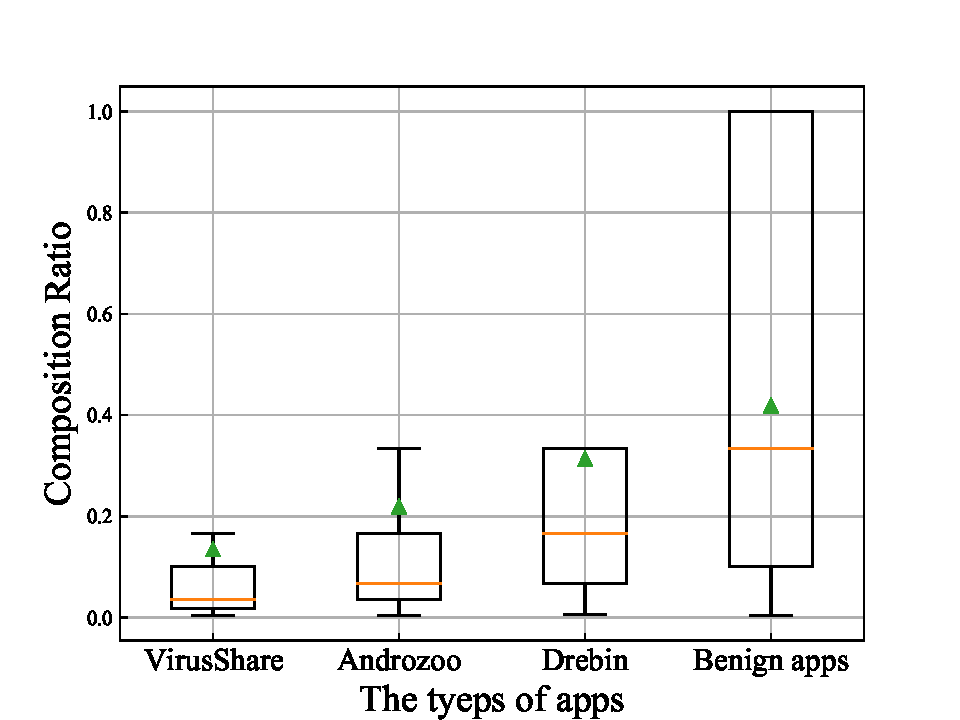
\includegraphics[scale=0.4]{./figures/com_ratio_dangerous_box.pdf}
    } &
    \subfigure[Custom permissions]{ %
      \label{fig:boxplot_custom}
      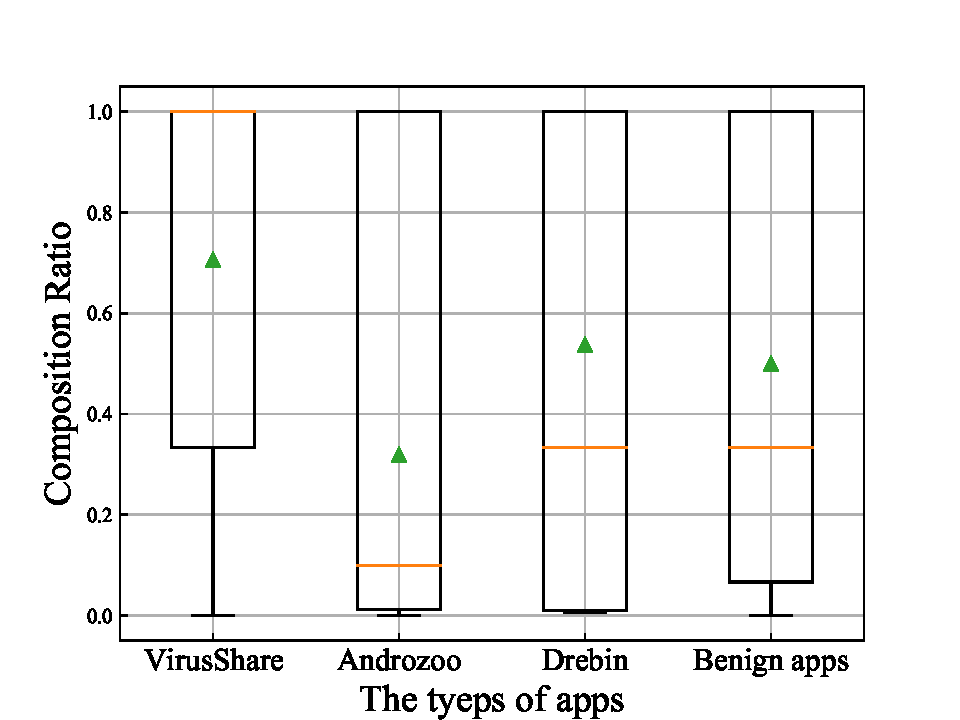
\includegraphics[scale=0.4]{./figures/com_ratio_custom_box.pdf}
    } \\
  % }
  \end{tabular}
  \caption{Box plots of the CR of permission pairs required by benign apps and malware samples. The orange lines and green triangles mean the median and the mean, respectively.}
  \label{fig:boxplot}
\end{figure*}
In order to satisfy the above requirements, in this paper, we propose Android malware detection based on the CR of permission pairs
% We focus on the fact that the ratio of a permission pair to all pairs tends to be small in malware samples compared with benign apps.
The CR is defined as a ratio of a permission pair to all pairs in an app.
% We focus on the fact that the CR tends to be small in malware because of unnecessary permissions.
We focus on the fact that the CR tends to be small in malware compared with benign apps.
This is because malware samples tend to require unnecessary permissions to imitate benign apps.
% We call this ratio Composition Ratio (CR) of permission pairs.
% As a result, there exists difference of the CR between benign apps and malware.
% In other words, the CR of malware tends to be smaller than that of a benign app.
% The CR is a numerical value which means how permission pairs are required with other ones.
% For example, suppose that an app requires five permissions in its manifest file.
% In this case, since the number of permission pairs is 10, the CR is $0.1 = \frac{1}{10}$.
Our scheme calculates CRs of permission pairs from four aspects, namely Android Permission (AP), Dangerous Permission (DP), Custom Permission (CP), and all permissions.  
% Our scheme calculates CRs based on pairs of four types of permissions, namely Android Permission (AP), Custom Permission (CP), Dangerous Permission (DP), and all permissions.  
Although more than 300 permissions are predefined in Android specifications \cite{androidpermissionslist}, our scheme regards the predefined permissions other than DPs as APs.
DPs consist of 24 permissions that enable accessing sensitive data such as personal information in users' devices and are also specified in the specifications.
CPs are permissions defined by developers while they are not in the specifications.
All permissions are made up of all the above permissions, namely APs, DPs, and CPs.
In our scheme, except for pairs generated from all permissions, pairs are composed only of the same kind of permissions.
For example, if an app requires two APs (AP1 and AP2), three DPs (DP1, DP2, and DP3), and no CP, an AP based pair (AP1:AP2) and three DP based ones (DP1:DP2, DP2:DP3, and DP3:DP1) are created.
% In this case, the AP based CR and the DP based one are $1.0 = \frac{1}{1}$ and $0.33 = \frac{1}{3}$, respectively.  
In this case, the CRs based on APs and DPs are $1.0 = \frac{1}{1}$ and $0.33 = \frac{1}{3}$, respectively.  
As for the CR based on CP in this app, 0.0 is specially assigned to it because there is no CP based pair.
Meanwhile, the CR based on all permission is $0.1 = \frac{1}{10}$ because there exist 10 pairs in total.
Thus, the CRs based on APs, DPs, CPs, and all permissions are 1.0, 0.33, 0.0, and 0.1, respectively.
% Thus, four types of CRs are obtained for pairs in an app.
The CRs are common among the same type of pairs.
For instance, 0.33 is assigned to every DP based pair.
% DP1:DP2, DP2:DP3, and DP3:DP1.

To leverage the tendencies of the CR for detection, four CRs based databases are constructed for each label of training databases (benign apps and malware).
In other words, eight databases are prepared in total.
For each app, we calculate eight similarity scores on the basis of corresponding databases.
% Out of eight scores, score for benign apps and one for malware on the basis of the databases.
% For each app, we calculate a similarity score for benign apps and one for malware on the basis of the databases.
By doing this, even if malware requires unnecessary permissions, useful features of them can be obtained from a new aspect except for the frequency.
Thus, our scheme can satisfy ``Stability''.
Finally, as features in ML, our scores are fed into classifiers such as Random Forest (RF) \cite{breiman2001random}, Support Vector Machine (SVM) \cite{cortes1995support}, and Adaboost \cite{freund1997decision} for detection.
% The proposed scheme calculates eight scores on the basis of the CR based similarity.
Since our scheme utilizes just eight-dimensional features, it can realize reducing computational cost of training and compatibility with other features, which results in satisfaction of ``Efficiency''.  
Besides, our scores can quantitatively offer clear information that what types of permission pairs dictate detection results.
% Our scores are easy to be understood because information about required permission pairs can be expressed as eight simple scores.
Thus, since understandable information are provided for human, the proposed scheme also meets ``Intelligibility''.
Since all the requirements can be met, our scheme is more suitable for practical use.

In what follows, we first validate usefulness of the CR.  
After that, the overview of the proposed scheme and its algorithms are explained in detail.

% In what follows, we first explain the CR of permission pairs.  
% After that, we validate usefulness of the CR.
% Finally, the overview of the proposed scheme and its algorithms are explained in detail.
% \subsection{Composition Ratio} 

\subsection{Validation of Usefulness of Composition Ratio of pairs} 
To validate that the CR of permission pairs are useful in malware detection, we investigated the distribution of the CR of permission pairs in apps by using box plot.
\myfigurename~\ref{fig:boxplot} shows the box plots of the CR of permission pairs required by benign apps and malware samples in three types of dataset.
In this investigation, 4,000 malware samples were randomly selected from each of Drebin \cite{arp2014drebin}, Androzoo \cite{allix2016androzoo}, and VirusShare \cite{virusshare} datasets.
Similarly, 4,000 benign apps were also randomly selected from benign dataset provided by Androzoo.
In \myfigurename~\ref{fig:boxplot}, there exist four box plots in terms of four types of permissions.
As shown in \myfigurename~\ref{fig:boxplot_all}, \myfigurename~\ref{fig:boxplot_android}, and \myfigurename~\ref{fig:boxplot_dangerous}, in terms of all permissions, AP, and DP, there exist clear differences of the distribution between benign apps and malware samples.  
The CRs of malware samples from VirusShare, Androzoo, and Drebin are distributed within a range of 0.0 to 0.4.
In particular, the variance of the CRs of malware samples from VirusShare is very small, which means that they tend to require more permissions.
Moreover, it can be seen that the CRs in Drebin are also distributed in a narrow range, which means the CR is effective in detecting old malware.
Meanwhile, the CRs of benign apps are more widely distributed than those of malware samples in the three types of permissions.
Average value in benign apps are also higher than the ones in malware sources.
With regard to CP, as shown in \myfigurename~\ref{fig:boxplot_custom}, the CRs are widely distributed in all types of apps.
Therefore, obvious difference is not observed compared with three other types of permissions.
However, since there exist differences of the median and the mean between two types of apps to some extent, we concluded that the CRs of CP based pairs can also be effective in detection.
These results demonstrate that the CRs of permission pairs are useful to distinguish benign apps from malware samples.
From these results, we concluded that using the CRs of four types of permission pairs are competent to correctly detect malware samples without relying on their frequencies.

\subsection{Algorithm}
In this section, we describe the algorithm of the proposed scheme.
\myfigurename~\ref{fig:overview} shows the overview of the proposed scheme.
\begin{figure*}[t]
  \centering
  \includegraphics[scale=0.80]{./figures/overview_pair.pdf}
  % \includegraphics[scale=0.8]{./figures/overview/overview_pair.pdf}
  \caption{The overview of the proposed scheme.}
  \label{fig:overview}
\end{figure*}
The proposed scheme has two main phases, namely, 1) CR based database construction, 2) the proposed score calculation.
In the first phase, for each label, CR based databases are constructed depending on permission types.
To capture more detailed features of apps, the proposed scheme constructs the four databases from the perspective of APs, DPs, CPs, and all permissions for each label.
In the second phase, for each app, eight scores are calculated on the basis of corresponding databases constructed in the first phase.
Finally, the eight scores are used as features for ML.
The detailed algorithm of each operation is presented in the next section.

\makeatletter
\newcommand{\multiline}[1]{%
  \begin{tabularx}{\dimexpr\linewidth-\ALG@thistlm}[t]{@{}X@{}}
    #1
  \end{tabularx}
}
\makeatother
\newcommand{\TRAINDATASET}{D_{\mathrm{training}}} % 
\newcommand{\PTYPE}{pt} % 
\newcommand{\DB}{D^{\PTYPE, l}} % 
% \newcommand{\DBALL}{DB^{\mathrm{all}}} % 
\newcommand{\DBA}{DB^{\mathrm{android}}} % 
\newcommand{\DBD}{DB^{\mathrm{dangerous}}} % 
\newcommand{\DBC}{DB^{\mathrm{custom}}} % 
\newcommand{\TRAINAPP}[1]{ta_{#1}} % 
\newcommand{\TRAINPERMISSIONSET}{TP_{\PTYPE, l}} % 
\newcommand{\PERMISSIONSET}[1]{P^{\PTYPE, l}_{#1}} % 
\newcommand{\PERMISSIONPAIRSET}[1]{P^{\mathrm{pair}}_{#1}} % 
\newcommand{\CRATIO}[1]{cr_{#1}} % 
\newcommand{\PAIR}{(p_j, p_k)} % 
\subsubsection{Composition Ratio Based Database Construction}
Algorithm \ref{alg1} shows CR based database construction.
As an input, Algorithm \ref{alg1} needs a set $\TRAINPERMISSIONSET = \{\PERMISSIONSET{\TRAINAPP{1}}, ..., \PERMISSIONSET{\TRAINAPP{i}}, ..., \PERMISSIONSET{\TRAINAPP{N}}\}$, which consists of $\PERMISSIONSET{\TRAINAPP{i}}$ which is a set of permissions required by $\TRAINAPP{i}$.  
Note that $\TRAINAPP{i}$ means an app in the training dataset, and the total number of $\TRAINAPP{i}$ is $N$.
Furthermore, $\PTYPE$ and $l$ denote a type out of four permission types and a label of a training dataset, respectively.
% Let $\PERMISSIONSET{\TRAINAPP{i}}$ denote a set of permissions required by an app $\TRAINAPP{i}$.
Algorithm~\ref{alg1} outputs a CR based database depending on $\PTYPE$ and $l$.
Let $\DB$ denote an output database.
If an input is a set of APs required by benign apps, $D^{\mathrm{AP, ben}}$ which means a database of CRs based on AP pairs for benign apps is constructed.
For each $\TRAINAPP{i}$, $\PERMISSIONPAIRSET{\TRAINAPP{i}}$ which means a set of permission pairs in $\TRAINAPP{i}$ is created on the basis of $\PERMISSIONSET{\TRAINAPP{i}}$.
After that, each pair $\PAIR \in \PERMISSIONPAIRSET{\TRAINAPP{i}}$ and $\CRATIO{\PAIR}$ which is the CR of pairs are registered with $\DB$ as a key and a value, respectively.
If $\PAIR$ has already existed in $\DB$, $\CRATIO{\PAIR}$ are added to existing values that corresponds to $\PAIR$.
Finally, every value in $\DB$ are divided by the total number of the training dataset, $|\TRAINPERMISSIONSET|$, which means calculating the average CR in the training dataset.
Similarly, Algorithm~\ref{alg1} is repeatedly conducted so as to create databases that corresponds to other permission types. 
Finally, four types of databases are constructed for each label, which means that eight databases are obtained in total.  
\begin{algorithm}[t]
  \caption{CR Based Database Construction}
  \label{alg1}
  \begin{algorithmic}[1]
  % \Require $\TRAINDATASET = \{\TRAINAPP{1}, ..., \TRAINAPP{i}, ..., \TRAINAPP{N_{app}}\}$
  % \Require $\PERMISSIONSET{\TRAINAPP{i}} = \{p_1, ..., p_j, ..., p_m\}$ from $\TRAINAPP{i}$
    \Require $\TRAINPERMISSIONSET = \{\PERMISSIONSET{\TRAINAPP{1}}, ..., \PERMISSIONSET{\TRAINAPP{i}}, ..., \PERMISSIONSET{\TRAINAPP{N}}\}$ 
    \Ensure A database $\DB$ of $pt$ and $l$ %$\TRAINPERMISSIONSET$ %, \DBA, \DBD, \DBC$
  \For{each $\PERMISSIONSET{\TRAINAPP{i}} \in \TRAINPERMISSIONSET$}
    % \State Extract $\PERMISSIONSET{\TRAINAPP{i}} = \{p_1, ..., p_j, ..., p_m\}$ from $\TRAINAPP{i}$ 
    \State Create $\PERMISSIONPAIRSET{\TRAINAPP{i}} = \{(p_1, p_2), ..., (p_j, p_k)\}$ from $\PERMISSIONSET{\TRAINAPP{i}}$ 
    % \State \multiline{For every type of pairs, a corresponding database is constructed.} 
    \For{each $\PAIR \in \PERMISSIONPAIRSET{\TRAINAPP{i}}$}
    % \State{For every permission $p_j$, }
      \If{$|\PERMISSIONPAIRSET{\TRAINAPP{i}}| \neq 0$}
        \State{$\CRATIO{\PAIR} = \frac{1}{|\PERMISSIONPAIRSET{\TRAINAPP{i}}|}$}
      \Else
        \State{$\CRATIO{\PAIR} = 0$}
      \EndIf
      \If{$\PAIR$ exists in $\DB$}
        \State $\DB_{\PAIR} += \CRATIO{\PAIR}$ 
      \Else
        \State $\DB_{\PAIR} = \CRATIO{\PAIR}$ 
      \EndIf
    \EndFor 
  \EndFor 
  \State Divide every value in $\DB$ by $|\TRAINPERMISSIONSET|$
  % \State \Return $\DB_{\PAIR}$
  \State \Return $\DB$
  \end{algorithmic}
\end{algorithm} 
\subsubsection{Proposed Score Calculation}
\newcommand{\APP}[1]{a_{#1}} % 
\newcommand{\MDB}{D^{pt, \mathrm{mal}}} % 
\newcommand{\BDB}{D^{pt, \mathrm{ben}}} % 
\newcommand{\SMAL}{s_{\mathrm{mal}}} % 
\newcommand{\SBEN}{s_{\mathrm{ben}}} % 
\newcommand{\MSCORE}{MS^{pt}_{\APP{i}}} % 
\newcommand{\BSCORE}{BS^{pt}_{\APP{i}}} % 
\newcommand{\NUMPERM}{N'} % 
\newcommand{\PERMISSIONSETTWO}[1]{P^{\PTYPE}_{#1}} % 
\begin{algorithm}[t]
  \caption{The Proposed Score Calculation}
  \label{alg2}
  \begin{algorithmic}[1]
    \Require $\PERMISSIONSETTWO{\APP{i}} = \{p_1, ..., p_j, ..., p_{\NUMPERM}\}$ of an app $\APP{i}$
  % \Ensure feature vector $V_{\TRAINAPP{i}}$
  \Ensure $\MSCORE$ and $\BSCORE$
  % \For{each $\TRAINAPP{i} \in \TRAINDATASET$}
    \State Create $\PERMISSIONPAIRSET{\APP{i}} = \{(p_1, p_2), ..., (p_j, p_k), ..., (p_{\NUMPERM-1}, p_{\NUMPERM})\}$ 
    % \State \multiline{For every type of pairs, a corresponding database is constructed.} 
    \For{each $(p_{j}, p_{k}) \in \PERMISSIONPAIRSET{\APP{i}}$}
    % \State{For every permission $p_j$, }
    \State{Initializing similarity values $\SMAL=0$, $\SBEN=0$}
      \If{$|\PERMISSIONPAIRSET{\TRAINAPP{i}}| \neq 0$}
        \State{$\CRATIO{(p_{j}, p_{k})} = \frac{1}{|\PERMISSIONPAIRSET{\APP{i}}|}$}
      \Else
        \State{$\CRATIO{\PAIR} = 0$}
      \EndIf
        \If{$(p_{j}, p_{k})$ exists only in $\MDB$}
        \State $\SMAL= 1$ 
        \ElsIf{$(p_{j}, p_{k})$ exists only in $\BDB$}
        \State $\SBEN = 1$ 
          % \State $\DBALL = \CRATIO{all}{(p_{i}, p_{j})}$ 
        \ElsIf{$(p_{j}, p_{k})$ is both in $\BDB$ and $\MDB$}
        \State $\SMAL = 1-|\CRATIO{\PAIR} - \MDB_{\PAIR}|$ 
      \State $\SBEN = 1-|\CRATIO{\PAIR} - \BDB_{\PAIR}|$ 
          % \State $\DBA_{(p_{i}, p_{j})} = 1$
        \EndIf
      \If{$\SMAL > \SBEN$}
       \State $\MSCORE += \SMAL$
      \ElsIf{$\SMAL < \SBEN$}
        \State $\BSCORE += \SBEN$
        % \Else:
        % \State{$(p_{i}, p_{j})$ exists both in $\BDBALL$ and $\MDBALL$}
      \EndIf
    \EndFor 
  % \EndFor 
  \State \Return $\MSCORE$ and $\BSCORE$
  \end{algorithmic}
\end{algorithm}
The proposed scores are calculated for every app in both a training dataset and testing one so as to create feature vectors.
Algorithm \ref{alg2} shows the proposed score calculation.
In Algorithm~\ref{alg2}, two scores, namely Malicious Score (MS) $\MSCORE$ and Benign Score (BS) $\BSCORE$ are calculated for an app $\APP{i}$ depending on $\PTYPE$.
Note that $\MSCORE$ and $\BSCORE$ indicate a similarity score with malware and benign apps, respectively.  
The larger each score is, the higher the degree of similarity is. 
For each app $\APP{i}$, eight scores are calculated in total.
% For simplicity, the procedure of calculating the score for APs is described in this section.
As an input, Algorithm \ref{alg2} requires $\PERMISSIONSETTWO{\APP{i}}$ that denotes a set of permissions in $\APP{i}$.
First of all, a set of permission pairs, $\PERMISSIONPAIRSET{\APP{i}} = \{(p_1, p_2), ..., \PAIR, ..., (p_{\NUMPERM-1}, p_{\NUMPERM})\}$ is created from $\PERMISSIONSETTWO{\APP{i}}$.
Note that $\NUMPERM$ means the number of permissions in $\APP{i}$.
After that, $\CRATIO{\PAIR}$ is compared with a value in $\MDB$ and $\BDB$.
Here, $\MDB$ represents a CR based database of malware in terms of $\PTYPE$.
Similarly, $\BDB$ means the database of benign apps.
If $\PAIR$ exists only in $\MDB$, a similarity value for malware, $\SMAL=1$.
Meanwhile, if $\PAIR$ exists only in $\BDB$, a benign similarity value, $\SBEN=1$.
In the case where $\PAIR$ exists both in $\MDB$ and $\BDB$, $\SMAL$ and $\SBEN$ are calculated on the basis of absolute values of differences between $\CRATIO{\PAIR}$ and statistical values in the databases, namely $|\CRATIO{\PAIR} - \MDB_{\PAIR}|$ and $|\CRATIO{\PAIR} - \BDB_{\PAIR}|$, respectively.
% Similarly, $\SBEN$ is also determined by calculating $|\CRATIO{\PAIR} - \BDB_{\PAIR}|$.
The smaller absolute values are, the higher $\SMAL$ and $\SBEN$ are, which means high similarities.
Finally, $\MSCORE$ and $\BSCORE$ are calculated depending on magnitude relationship of $\SMAL$ and $\SBEN$.
If $\SMAL$ is higher than $\SBEN$, $\SMAL$ is added to $\MSCORE$; otherwise $\SBEN$ is added to $\BSCORE$.  
Similarly, $\MSCORE$ and $\BSCORE$ are calculated on the basis of other types of permission pairs.
Thus, the eight scores are obtained for $\APP{i}$.
Finally, they are fed into a ML based classifier as feature vectors for training and testing.  

\section{Evaluation Results and Discussion} \label{sec:simulation}
% \subsection{Evaluation Setting}
% \subsubsection{Evaluation Metric and Environment}
\subsection{Dataset}
\mytablename~\ref{tab:dataset} shows datasets of APK files used in our simulation.
Benign apps were obtained from Androzoo \cite{allix2016androzoo} distributed between 2017 and 2020 (2017--2020). 
Malware samples were collected from Drebin (2010--2012) \cite{arp2014drebin}, Androzoo (2017--2020), and VirusShare (2018--2020) \cite{virusshare}.
% In order to conduct our simulation on the basis of recent tendency, we used latest datasets collected between 2017 and 2020.
In our evaluation, we used only the apps that require more than one permissions including all permissions because our work focus on appraising permission pairs based schemes.
With regard to Androzoo and VirusShare, as a testing dataset, we randomly selected 1,500 benign apps and 1,500 malware samples from all of the benign dataset and all of the malware dataset, respectively.
% Furthermore, in our simulation, there exist 2 types of training datasets, namely, a training dataset used by the detection method and one used by attackers.
Besides, we constructed the training dataset by randomly selecting 6,000 benign apps and 6,000 malware samples from the rest of them.
On the other hand, in terms of malware samples in the Drebin dataset, 1,000 apps and 3,000 apps are randomly selected as testing malware samples and training ones, respectively.
This is because the total number of Drebin malware samples in our dataset is 4364.
As for benign apps, 1,000 testing dataset and 3,000 training one are also randomly selected to balance the number of datasets.
% As for K-NN, K is set to 3 because MaMaDroid achieves better detection performance with this parameter~\cite{onwuzurike2019mamadroid}.
\begin{table}[t]
  \begin{center}
    \caption{Datasets of APK files used in our evaluation.}
    \label{tab:dataset}
    \begin{tabular}{|c|c|c|c|c|} \hline
       & Source & Period & Testing & Training \\ \hline 
      \multirow{3}{*}{Malware} & Drebin \cite{arp2014drebin} & 2010--2012 & 1,000 & 3,000\\ \cline{2-5}
                               & Androzoo \cite{allix2016androzoo}& 2017--2020 & 1,500 & 6,000\\ \cline{2-5}
                               & VirusShare \cite{virusshare} & 2018--2020 & 1,500 & 6,000\\ \hline
      Benign apps & Androzoo \cite{allix2016androzoo}& 2017--2020 & 1,500 & 6,000  \\ \hline
      Benign apps & \multirow{2}{*}{Androzoo \cite{allix2016androzoo}} & \multirow{2}{*}{2017--2020} & \multirow{2}{*}{1,000} & \multirow{2}{*}{3,000 } \\ 
      for Drebin & & & & \\ \hline
    \end{tabular}
  \end{center}
\end{table}

% \subsection{Combination of Proposed Scores}
% % $BDs0F$N%9%3%"$NAH$_9g$o$;$NHf3S(B

\subsection{Comparison with conventional schemes} \label{sec:comparison}
\subsubsection{Detection Performance} \label{sec:detection_performance}
\begin{table*}[t]
  \begin{center}
    \caption{Detection performance of the conventional schemes and the proposed schemes.}
    \label{tab:detection_performance} 
    \begin{tabular}{|c|c|c|c|c|c|c|c|c|c|c|c|c|} 
    % \begin{tabular}{ccccccccccccc} 
      \hline
      % \wcline{1-13}
      \multirow{3}{*}{\textbf{Scheme}} & \multicolumn{3}{c|}{Drebin (2010--2012) } & \multicolumn{3}{c|}{Androzoo (2017--2020)} & \multicolumn{3}{c|}{VirusShare (2018--2020)}& \multicolumn{3}{c|}{Mixed dataset}\\ \cline{2-13}
                                       & ACC  & TPR & FPR & ACC & TPR & FPR & ACC & TPR & FPR & ACC & TPR & FPR \\ 
                                       & (\%) & (\%) & (\%) & (\%) & (\%) & (\%) & (\%) & (\%) & (\%) & (\%) & (\%) & (\%) \\ \hline 
      Prop. (RF)  & \textbf{97.3} & 97.7 & 3.1 & \textbf{80.4} & 80.0 & 19.2 & 91.2 & 90.3 & 7.8 & 84.0 & 82.4 & 14.3 \\ 
      Prop. (SEL)  & 97.2 & 97.5 & 3.1 & 80.2 & 79.8 & 19.3 & \textbf{91.3} & 90.3 & 7.7 & \textbf{84.2} & 81.4 & 12.9 \\ 
      PermPair \cite{arora2019permpair}  & 89.1 & 97.8 & 19.6 & 50.1 & 99.9 & 99.6 & 50.0 & 99.9 & 99.8 & 50.1 & 99.9 & 99.6 \\ 
      BVBS \cite{liu2014two} & 96.8 & 96.9 & 3.3 & 79.7 & 78.9 & 19.4 & 91.2 & 90.5 & 8.0 & 83.5 & 81.9 & 14.9 \\ 
      \hline
      % \wcline{1-13}
    \end{tabular}
  % }
  \end{center}
\end{table*} 
% $BDs0F$O(B8$B8D$NFCD'$G!"=>Mh$HF1Ey0J>e$N8!CN@:EY$G$"$k$3$H(B
% PermPair$B$OIQEY$K4p$E$$$?%G!<%?%Y!<%9$rMQ$$$k$3$H$G!"I=8=NO$H2r@O$N$7$d$9$5$ONI$$$,!"8!CN@:EY$KCWL?E*$J7gE@$,$"$k!#(B
% BVBS $B$O8!CN@:EY$ODs0F$H$[$\F1Ey$G$"$C$?$,!"FCD'%Y%/%H%k$,>iD9$G$"$j!"2r<a$b$7$E$i$$!#(B
% $B$=$l$KHf$Y$F!"Ds0F$O!"%7%s%W%k$J%9%3%"$H%G!<%?%Y!<%9$r6n;H$9$k$3$H$G!"2r<a$N$7$d$9$5$H8!CN@:EY$rN>N)$7$F$$$k!#(B
% $B2r<a@-$N$"$k$3$H$rMxMQ$7$FJ,@O$r$9$k$h(B
% $B7W;;;~4V$J$I$O<!$N>O$GHf3S$9$k$h(B 
To evaluate the detection performance against old malware samples and recent ones, we evaluate ACCuracy (ACC), True Positive Rate (TPR), and False Positive Rate (FPR) with real dataset.
ACC, TPR, and FPR are calculated as
\begin{equation}
  \mathrm{ACC} = \frac{\mathrm{TP}+\mathrm{TN}}{\mathrm{TP} + \mathrm{TN} + \mathrm{FP} + \mathrm{FN}}, 
\end{equation}
\begin{equation}
  \mathrm{TPR} = \frac{\mathrm{TP}}{\mathrm{TP + FN}},
\end{equation}
\begin{equation}
  \mathrm{FPR} = \frac{\mathrm{FP}}{\mathrm{FP + TN}},
\end{equation}
where TP, TN, FP, and FN denote the number of True Positive (malware samples are regarded as malware samples), True Negative (benign apps are regarded as benign ones), False Positive (benign apps are regarded as malware samples), and False Negative (malware samples are regarded as benign apps), respectively.  

We compare the proposed scheme with two conventional permission pairs based schemes, namely Boolean Vector Based Scheme (BVBS) \cite{liu2014two} and PermPair \cite{arora2019permpair}.
Note that in \cite{liu2014two}, although both a single permission and permission pairs are used for detection, we only evaluate results by using permission pairs.
This is because our focus is how to devise more practical detection with permission pairs.
In our evaluation, BVBS utilizes top 40 permissions which frequently appear in benign apps and malware samples in the training datasets in keeping with the number of permissions in \cite{liu2014two}.
In other words, BVBS utilizes 780 permission pairs as features for ML.
% $BAH$_9g$o$;$?$i$h$/$J$k$N$OEv$?$jA0$H=q$$$?J}$,NI$$!)(B
Furthermore, since it was reported that the RSBS \cite{liang2014permission} results in 55\% FP with permission pairs, that scheme is not adopted for comparison in our evaluation.

In terms of the proposed schemes, we evaluate two types of schemes.
The first one is a scheme with Random Forests (RF) \cite{breiman2001random} (hereinafter, this scheme is called ``Prop. (RF)'').
The reason why we adopt RF is that RF achieved fast training and more accurate detection performance compared with other classifiers in our preliminary experiments.
To fairly evaluate performance, BVBS also utilizes the RF classifier in our evaluation.
The other is a scheme that uses a technique called Stacking Ensemble Learning (SEL) for training of ML (This is called ``Prop. (SEL)'').
The SEL can improve predictive performance by combining outputs from multiple classification models.
In other malware detection methods \cite{vasan2020mthael, zhu2020sedmdroid}, the SEL is used to improve performance.
% , K-Neatest Neighbor (K-NN) \cite{cover1967nearest}, Support Vector Machine (SVM) \cite{cortes1995support}, and Adaboost \cite{freund1997decision}.

\mytablename~\ref{tab:detection_performance} shows detection performance of the conventional schemes and the proposed schemes.
In \mytablename~\ref{tab:detection_performance}, ACC, TPR, and FPR are appraised on every source. 
Furthermore, we evaluate detection performance of the four above schemes on a mixed dataset, which is composed of 6,000 benign apps and 6,000 malware samples from all sources.
Note that the benign apps and malware samples are randomly selected as with other datasets.
As shown in \mytablename~\ref{tab:detection_performance}, the proposed schemes achieves the highest ACC compared with PermPair and BVBS.
Moreover, the ACC of Prop. (SEL) is slightly higher than that of Prop. (RF), which means that SEL is useful for improving detection performance.
In terms of PermPair, although the ACC on Drebin is 89.1\%, the ACC values are 50.1\% and 50.0\% on Androzoo and VirusShare, respectively.
In particular, FPRs are 99.6\% and 99.8\% in Androzoo and VirusShare, respectively, which means that almost all the benign apps are misjudged as malware.
This is because PermPair is vulnerable to injecting unnecessary permissions in recent malware samples.
Recent malware samples tend to require permission pairs that are frequently required by benign apps, as shown in Section \ref{sec:shortcoming}.
As a result, the frequencies of most pairs in malware tend to be higher than those in benign apps.
These results show that frequency based databases get ineffective.
% Thus, when recent malware samples are utilized to create frequency based databases, databases are contaminated.
% PermPair considers permission pairs with high frequencies as important ones.
Therefore, PermPair cannot correctly identify benign apps.
% These results demonstrate that PermPair cannot deal with recent malware samples.

With regard to BVBS, it can achieve high detection performance as with Prop. (RF) and Prop. (SEL) whereas ACC is slightly low on all the four types of datasets.
Since boolean vectors express information about the presence of pairs by using boolean values (0 or 1), each pair is equally treated regardless of its frequency.
Hence, BVBS is insusceptible to the tendencies of recent malware, and its detection performance is not degraded.
This evaluation demonstrates that BVBS and the proposed scheme are capable to precisely classify apps into benign apps and recent malware, which means that they satisfy ``Stability''.
Although BVBS can fulfill ``Stability'', it cannot satisfy the other requirements.
In what follows, we compare the proposed scheme with BVBS in terms of aspects of ``Efficiency'' and ``Intelligibility''.

% \subsubsection{Resource Consumption}
% \begin{figure}[t]
  % \centering
  % 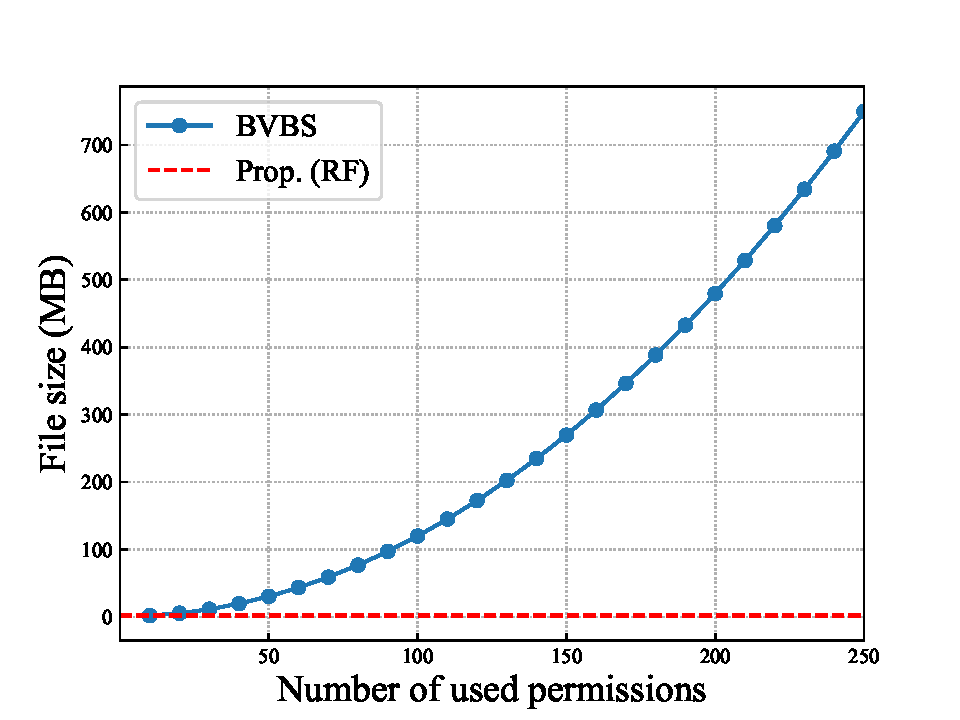
\includegraphics[scale=0.5]{./figures/csv_size.pdf}
  % \caption{The file size of feature vectors in the proposed method and BVBS.}
  % \label{fig:perm_size}
% \end{figure}
% $BDs0F$H=>Mh$G(BDB$B$N%5%$%:$rHf3S$9$k(B
% $BDs0F$H(BBVBS$B$NFCD'%Y%/%H%k$bHf3S$9$k(B
% $BDs0FJ}<0$HF1Ey$N@:EY$r=P$=$&$H$9$k$H!"(BBVBS$B$O?tI4G\$N<!85$K$J$k$?$a!"FCD'@8@.$K;~4V$,$+$+$k!#(B
% 250$B$N$H$-!A0l8D$"$?$jIC$@$C$?!#(B
% $B0lJ}$G!"Ds0F$O!"!A8D$N%Z%"$r9MN8$7$F$b!"FCD'%Y%/%H%k$N<!85$O0lDj$J$N$G!"AGAa$$FCD'@8@.$,2DG=$G$"$k!#(B
% $B$^$?!"(BBVBS$B$O!"%G!<%?NL$bB?$/$J$k!#(B
% $B@52rN($O!"9MN8$9$k%Q!<%_%C%7%g%s?t$rA}$d$;$P!"(BBVBS$B$NJ}$,<c439b$$$,!"J];}$9$k$Y$-%G!<%?$,B?$/$J$j$9$.$k!#(B
% $B<BMQLL$r9M$($k$H!"HFMQE*$J8!CN$N$?$a$KB?$/$NJ}<0$K4X$9$kFCD'$d%G!<%?$rJ]4I$9$k$3$H$+$i!"%j%=!<%9$O@aLs$9$kI,MW$,$"$k(B
% $BDs0F$O!"3X=,%G!<%?$O!A(B2.2MB$B$@$C$?!#(B

% \subsubsection{Training Time and Compatibility with Other Schemes}
\subsubsection{Computational Cost and Compatibility}
%  $B3X=,;~4V$ODs0F$,?tG\Aa$$!#(B
% Android$B%^%k%&%'%"$N8!CN$NJ,Ln$G$OB?$/$NJ}<0$,5!3#3X=,%Y!<%9$G$"$k$?$a!"B>$NJ}<0$NFCD'$HAH$_9g$o$;$F3X=,$5$;$k$3$H$b9M$($i$l$k!#(B
% $BNc$($P!"(BICC $B$J$I$O(B1000$B$N%*!<%@!<$G$"$k!#(B
% $B$=$N:]!"$?$C$?(B8$B<!85$7$+A}$($J$$$?$a!"Ds0FJ}<0$O3X=,;~4V$KBg$-$/1F6A$rM?$($k$3$H$O$J$/!"<BMQ2=$K$*$$$F$bHs>o$KNI$$(B.
% $B%Q!<%_%C%7%g%s$@$1$G$O8!CN$G$-$J$$$b$N$,$"$k$?$a!";~4V$,$+$+$kF0E*2r@O$N<jK!$rBhFsCJ3,$G$O9T$&2DG=@-$,9M$($i$l$k$,!"Bh0lCJ3,$G$N;~4V$r>/$J$/$9$k$3$H$O=EMW(B
As explained in Section \ref{sec:comparison} 1), BVBS is tolerant to the tendency of recent malware samples.
However, BVBS requires a high-dimensional feature vector to detect malware.
In this subsection, we first compare the proposed scheme with BVBS in terms of training time.
% Furthermore, to demonstrate the proposed scheme is superior to conventional schemes in computational cost, we also appraise runtime for feature construction and training of machine learning.
We ran our experiments on a machine with 2GHz Intel Core i5 and 16GB of RAM.
After evaluating training time, we discuss compatibility with other features in ML based schemes.  
Through the comparison and discussion, we show that only the proposed scheme satisfies ``Efficiency''.

We evaluate relationship between the number of used permissions and training time.
\myfigurename~\ref{fig:perm_time} shows the training time in the proposed methods and BVBS when the number of used permissions are changed.
In this evaluation, 6,000 benign apps and 6,000 malware samples are used in BVBS (RF), BVBS (SEL), Prop. (RF), and Prop. (SEL).
As shown in \myfigurename~\ref{fig:perm_time}, training time of BVBS (RF) and BVBS (SEL) exponentially increase as the number of permissions increases.
In particular, it takes up to 14,101s ($=$ 3h 55m) for training of 12,000 apps when 300 permissions are used for detection in BVBS (SEL).
In other words, BVBS (SEL) takes about 2,350 times longer than Prop. (SEL) in which training time is 6s.
\begin{figure}[t]
  \centering
  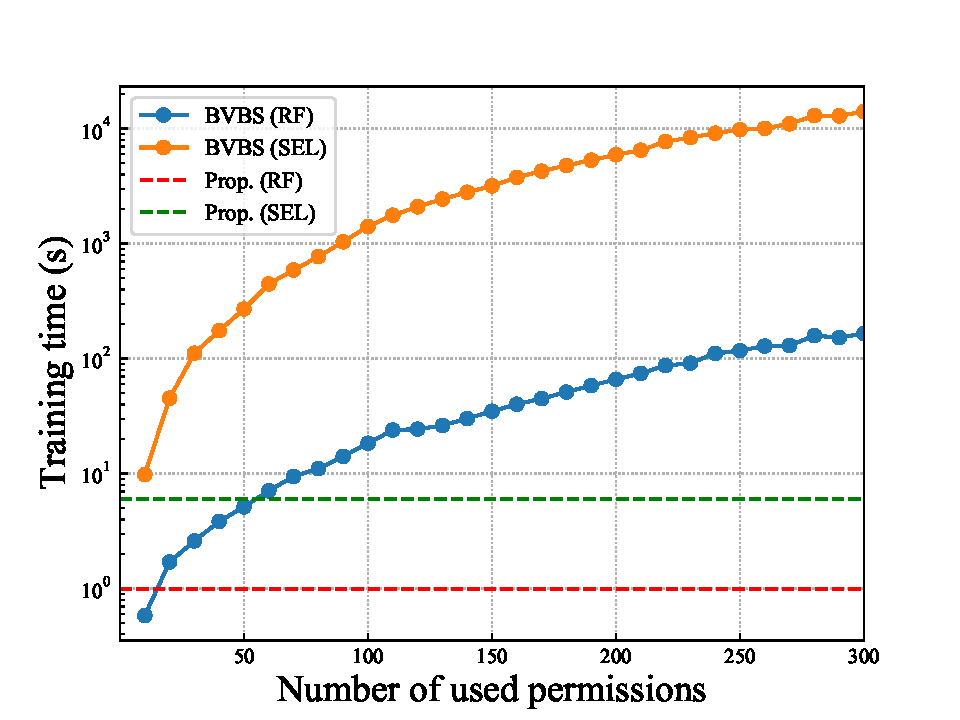
\includegraphics[scale=0.44]{./figures/csv_time.pdf}
  \caption{The training time in the proposed methods and BVBS when the number of used permissions are changed.}
  \label{fig:perm_time}
\end{figure}
\begin{figure}[t]
  \centering
  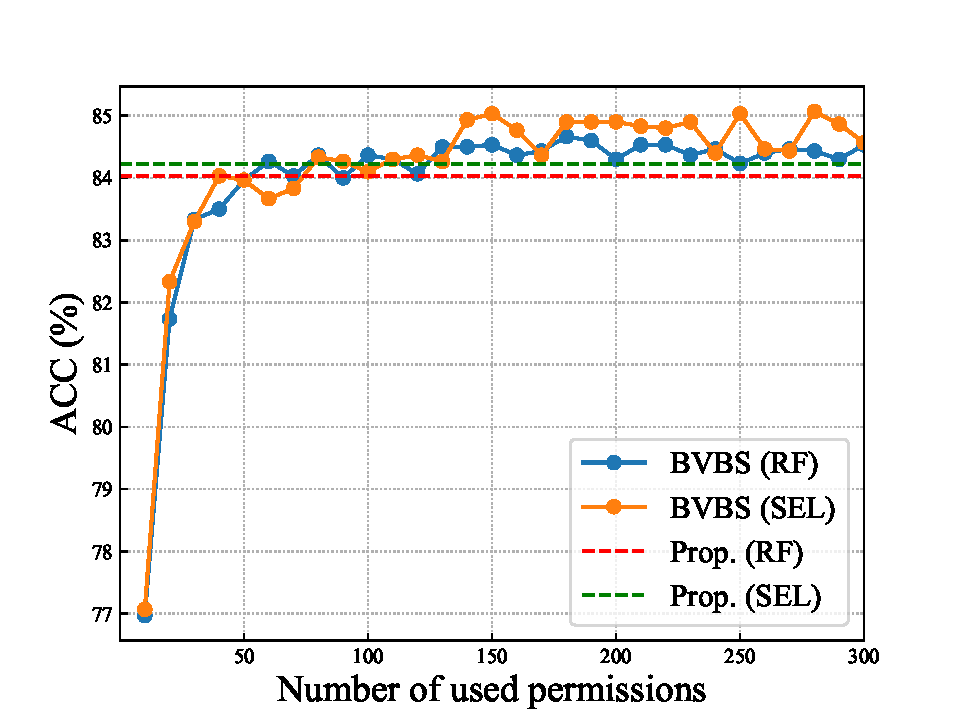
\includegraphics[scale=0.45]{./figures/perm_acc.pdf}
  \caption{The ACC of the proposed methods and BVBS when the number of used permissions are changed.}
  \label{fig:perm_acc}
\end{figure}

Meanwhile, \myfigurename~\ref{fig:perm_acc} shows the ACC of the proposed methods and BVBS when the number of used permissions are changed.
In \myfigurename~\ref{fig:perm_acc}, dotted lines of Prop. (RF) and Prop. (SEL) are just displayed as baselines.
As shown in \myfigurename~\ref{fig:perm_acc}, as the number of permissions increases, ACC values of BVBS and BVBS (SEL) are slightly increased whereas the improvement is trivial.
When 80 permissions are used in BVBS (3160 pairs are used), the ACC of BVBS and that of BVBS (SEL) are 84.36\% and 84.33\%, respectively, and these values are a little bit higher than that of Prop. (SEL), which is 84.2\%.
However, in this case, BVBS must utilizes 3160-dimensional vectors.
On the other hand, since our features are eight-dimensional, the proposed scheme reduces the feature dimensions by about 99\% with maintaining comparable detection accuracy.  
In the case where 280 permissions are used, whereas ACC of BVBS (SEL) is the best, already mentioned above, its computational cost of training gets huge.
In this case, the number of permission pairs is 39,060, and training time is 13,007s ($=$ 3h 36m).
% the dimensions of the feature vector is too large.
This result means that it is difficult to apply the SEL to BVBS in the practical situation although the SEL can ameliorate detection performance.

On the other hand, the training time of Prop. (RF) and that of Prop. (SEL) are 1s and 6s, respectively, in our evaluation.
Training time of the proposed scheme is independent of the number of used permission pairs because our feature vector is always eight-dimensional one regardless of the number of pairs. 
In our environment, the average elapsed time for calculating eight scores per an app is about $9.3 \times 10^{-4}$s.
In other words, our scheme can efficiently convert information about permission pairs into low-dimensional features.
% with maintaining almost comparable detection performance of BVBS.

Furthermore, because of the low-dimensional features, the proposed scheme is compatible with other ML based schemes.
In other words, our scheme is promising for hybrid detection with feature fusion.
The feature fusion means combining various features obtained from different aspects such as network traffic, API calls, ICC, and permissions so as to comprehensively detect various malware.
The feature fusion is frequently adopted in Android malware detection \cite{saracino2016madam, tao2017malpat, cai2018droidcat, arora2018ntpdroid}.
In \cite{saracino2016madam, arora2018ntpdroid}, permissions based features are combined with other features, and it is reported that the feature fusion is effective.
When the feature fusion is carried out, the dimensions of feature vectors inevitably get large.
For example, in \cite{xu2016iccdetector}, since more than 5,000-dimensional features can be used, it is desirable that additional features are low-dimensional ones.
If the dimensions get too large like BVBS, detection performance may not be versatile because of curse of dimensionality.
% In the practical use, there exist detection system that combines multiple detection schemes.
In particular, in the practical use, detecting malware comprehensively on the basis of various aspects is an ideal situation.
Thus, in light of such situations, our eight scores are effective and desirable features, which means that the proposed scheme is suitable for a practical detection system with the feature fusion unlike BVBS.
From these results, we concluded that the proposed scheme can satisfy not only ``Stability'' but also ``Efficiency''.
% \subsection{Runtime performance comparison}

% \subsubsection{Memory Consumption for Feature Vector Construction}
% \subsubsection{File Size of Feature Vector}
\subsection{Analysis of Detection Results} \label{subsec:analysis}
In this section, we demonstrate that our scores can offer useful information to understand detection results from a new aspect, namely the CR.
In other words, we show that the proposed scheme can satisfy ``Intelligibility''.
Our scheme can provide understandable information about detection results because permission pairs based information is converted into eight simple scores on the basis of the CR based databases.
The proposed scores and the CR based databases can help human to understand detection results as with PermPair.
On the other hand, it is difficult for BVBS to provide understandable information about detection results to human by using its feature vector.
% In the following subsections, we conduct true positive analysis and true negative analysis.
In the following subsections, we conduct detailed analysis and interpretation for tested apps that our scheme judged.

\subsubsection{Analysis for Detected Malware} 
\begin{figure*}[t]
  \centering
  \subfigure[Android permissions]{%
    \label{fig:score_a_mal}
    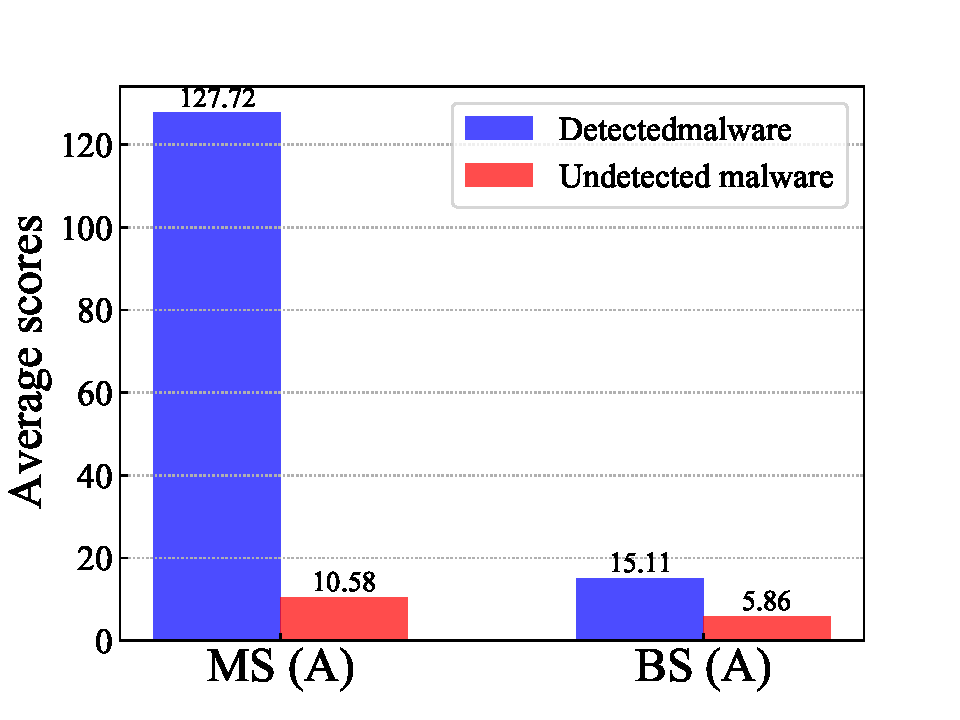
\includegraphics[scale=0.255]{./figures/bar_MS_(A)_BS_(A)_malware.pdf}
  } 
  \subfigure[Custom permissions]{ %
    \label{fig:score_c_mal} 
    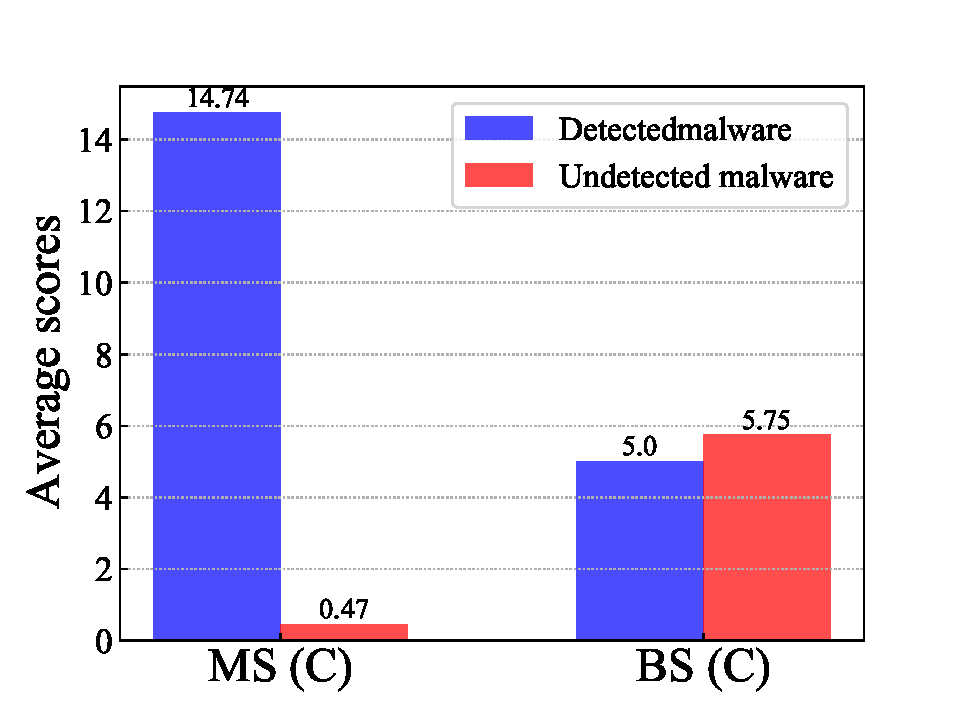
\includegraphics[scale=0.255]{./figures/bar_MS_(C)_BS_(C)_malware.pdf}
  } 
  \subfigure[Dangerous permissions]{ %
    \label{fig:score_d_mal} 
    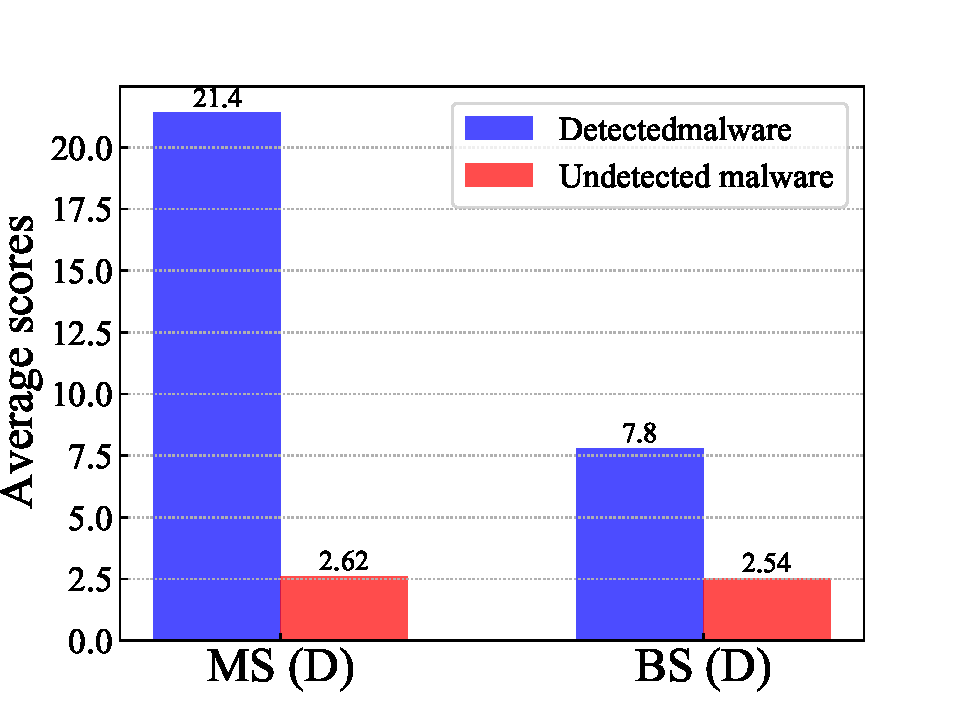
\includegraphics[scale=0.255]{./figures/bar_MS_(D)_BS_(D)_malware.pdf}
  } 
  \subfigure[All permissions]{ %
    \label{fig:score_all_mal} 
    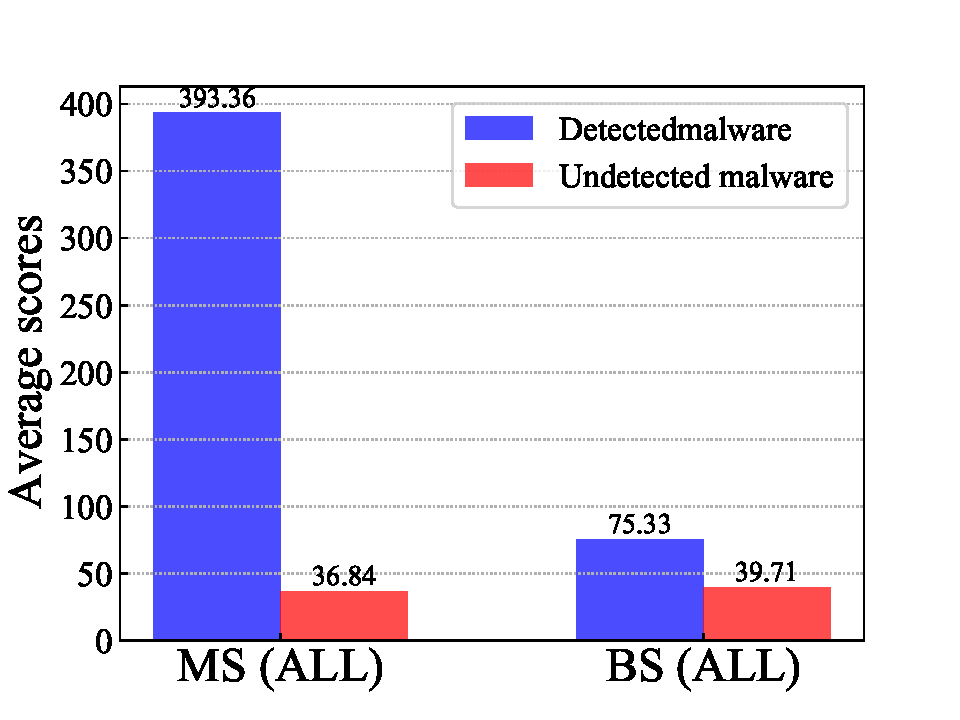
\includegraphics[scale=0.255]{./figures/bar_MS_(ALL)_BS_(ALL)_malware.pdf}
  } 
  \caption{Average proposed scores of detected malware samples and undetected ones. MS and BS mean Malicious Score and Benign Score, respectively. In terms of an alphabet and a word in parentheses after MS and BS, A, C, D, and ALL represent Android, Custom, Dangerous, and All permissions, respectively.}
  \label{fig:score_mal}
\end{figure*}
% $BA4A3%Q!<%_%C%7%g%s$r@EE*$KMW5a$7$F$$$J$$$3$H$,860x!#(B
% $B$3$l$i$N0-@-%"%W%j$O!"8"8B$rF0E*$K99?7$9$k$h$&$JJ}K!$r$H$k2DG=@-$,$"$k$?$a!"F0E*$K%Q!<%_%C%7%g%s$d(BAPI$B$N4X78$r2r@O$9$kJ}<0$J$I$,M-8z$G$"$k2DG=@-$,$"$k!#(B
\begin{figure*}[t]
  \centering
  \subfigure[Android permissions]{%
    \label{fig:android_p_dist_mal}
    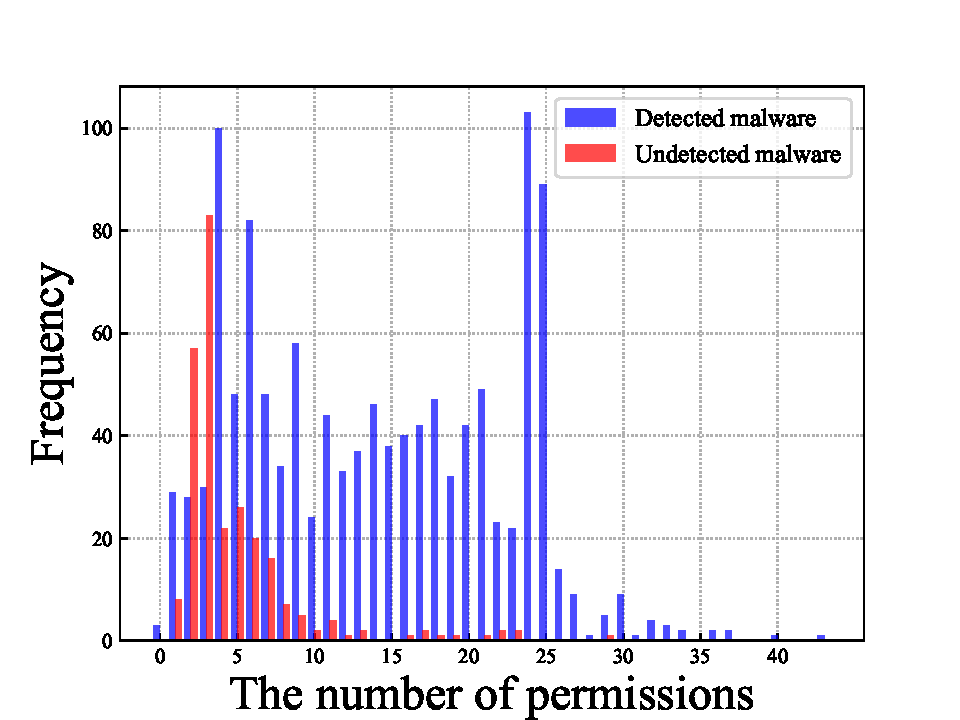
\includegraphics[scale=0.255]{./figures/malware_android_dist.pdf}
  } 
  \subfigure[Custom permissions]{ %
    \label{fig:custom_p_dist_mal} 
    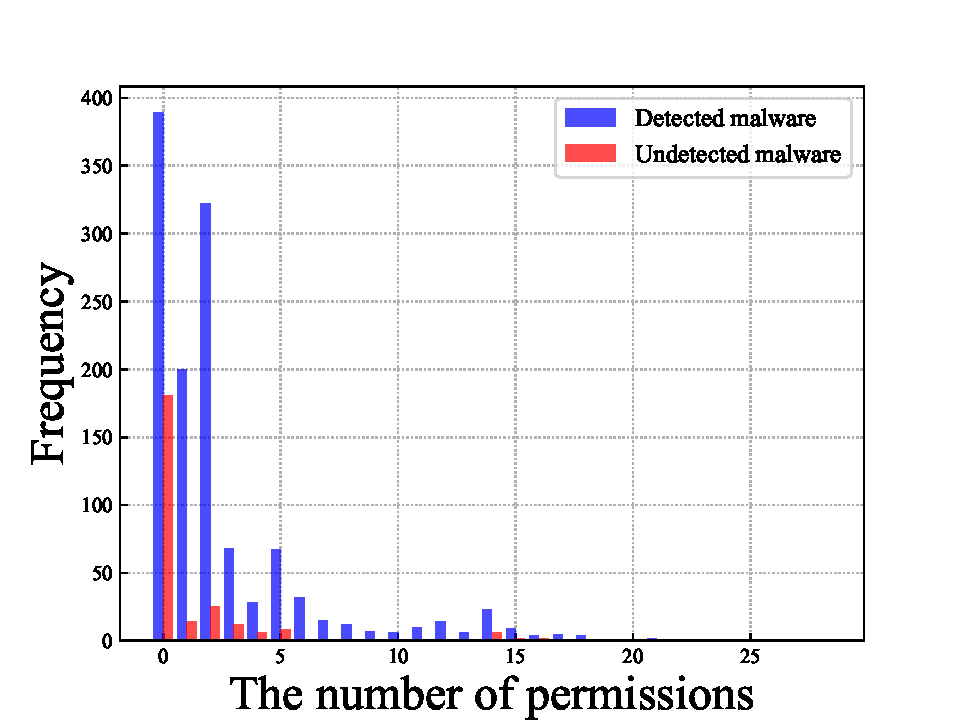
\includegraphics[scale=0.255]{./figures/malware_cumsum_dist.pdf}
  } 
  \subfigure[Dangerous permissions]{ %
    \label{fig:dangerous_p_dist_mal} 
    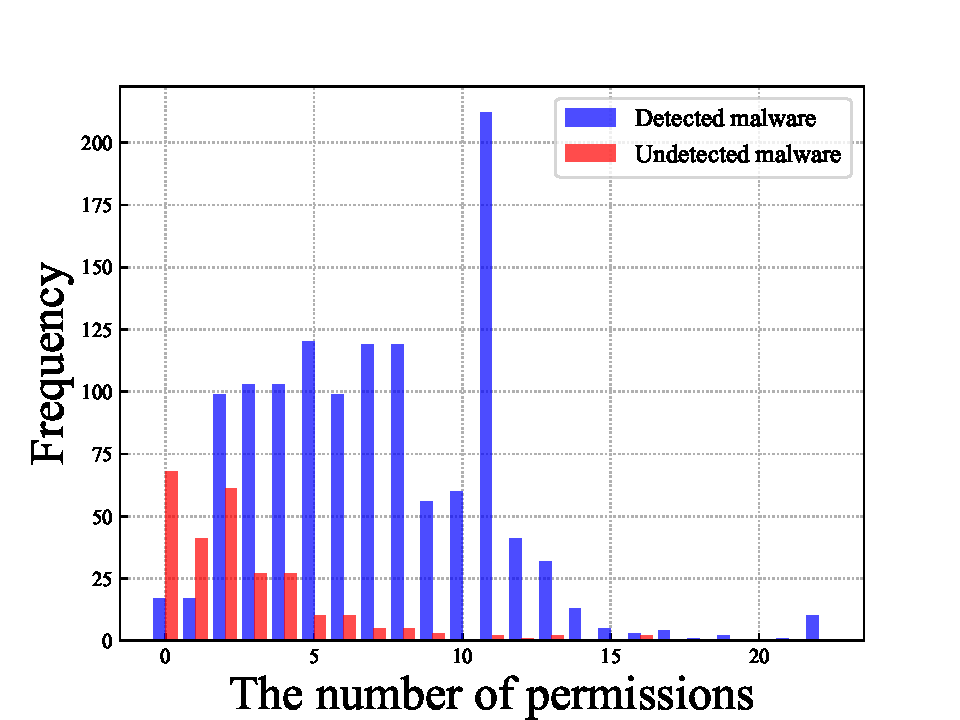
\includegraphics[scale=0.255]{./figures/malware_dangerous_dist.pdf}
  } 
  \subfigure[All permissions]{ %
    \label{fig:all_p_dist_mal} 
    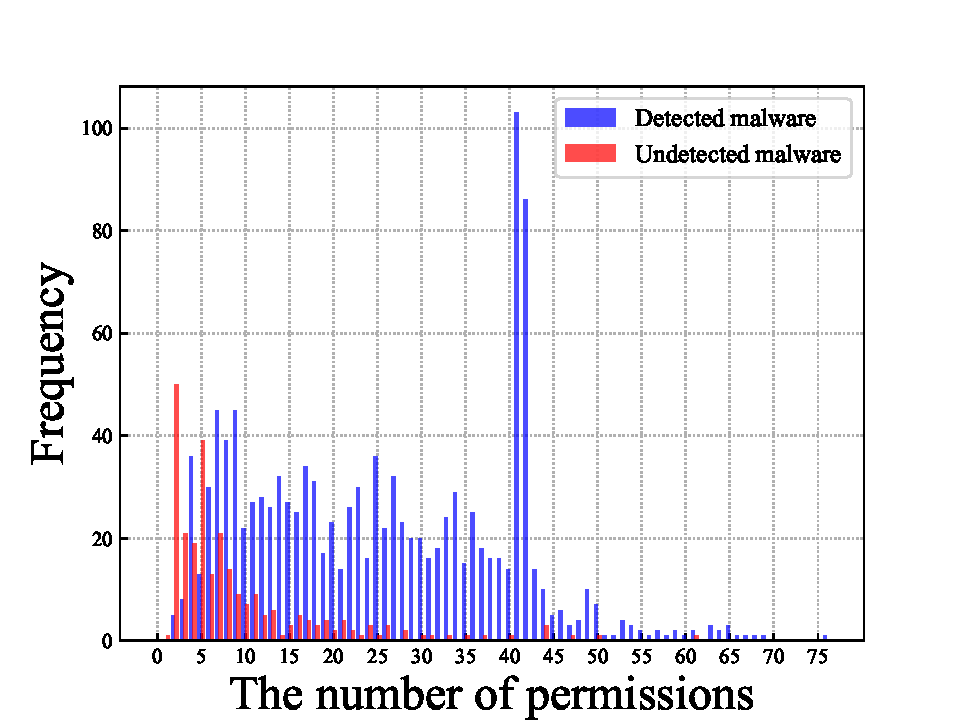
\includegraphics[scale=0.255]{./figures/malware_all_dist.pdf}
  } 
  \caption{Distribution of the number of permissions required by detected malware samples and undetected ones.}
  \label{fig:permission_distribution_mal}
\end{figure*}
% \subsubsection{True Positive Analysis}
% $BDs0F$@$1$G8!CN$G$-$?$b$N$N@bL@$r$9$k(B
In this subsection, we conduct analysis of malware samples that are judged by the proposed scheme.
\myfigurename~\ref{fig:score_mal} shows average proposed scores of detected malware samples and undetected ones.
Note that these average scores are calculated on the basis of 3,000 testing data, namely 1,500 benign apps and 1,500 malware samples from the mixed dataset.
As shown in \myfigurename~\ref{fig:score_mal}, there exist clear differences of our scores between detected malware samples and undetected ones.
In terms of detected malware samples (blue bars), the differences between MS and BS tend to be large. 
In particular, with regard to scores of malware in \myfigurename~\ref{fig:score_all_mal}, average MS (ALL) and BS(ALL) are 393.36, 75.33, respectively.
The difference between them is 318.03.
These results mean that the proposed scheme can calculate useful scores for identifying malware samples.

\subsubsection{Analysis for Undetected Malware}
On the other hand, as for undetected malware samples (red bars), it turns out that the differences between MS and BS are small compared with detected malware.
These small differences cause the proposed scheme to misjudge them as benign apps.
Through further analysis, we found the reason why these differences are small.
That is, misjudged malware samples tend to require fewer permissions compared with malware samples that are correctly judged.
As a result, since CRs of permission pairs get large, they affects our scores.
\myfigurename~\ref{fig:permission_distribution_mal} shows distribution of the number of permissions required by detected malware samples and undetected ones.
The used data are the same as the data in \myfigurename~\ref{fig:score_mal}.
As shown in \myfigurename~\ref{fig:permission_distribution_mal}, it can be seen that misjudged malware samples require fewer permissions in every type of permission.
In terms of CPs, as shown in \myfigurename~\ref{fig:custom_p_dist_mal}, even detected malware samples do not frequently require many CPs.
As for APs and DPs, malware samples tend to require many of them, as shown in \myfigurename~\ref{fig:android_p_dist_mal} and \myfigurename~\ref{fig:dangerous_p_dist_mal}.
Meanwhile, misjudged malware samples require fewer permissions.
Since benign apps tend to require only essential permissions, CRs of them tend to be large.
Thus, the CRs of misjudged malware samples are similar to those of benign apps, which results in incorrect scores of them.

We found a misjudged malware sample that has five permissions in total.
The malware has one CP and one DP, which means that permission pairs cannot be generated in the CP and the DP.
Since the proposed scheme is based on permission pairs, it cannot calculate MS (C), BS(C), MS (D), and BS(D) at all.
This malware requires INTERNET (INT) and WRITE\_EXTERNAL\_STORAGE (WES).
This pair is dangerous, because it enables the malware to install another malware in a device.
%  $B$3$3$G(BINT:WES$B$N%9%3%"=P$9(B
However, as for the pair INT:WES, $\SMAL$ and $\SBEN$ are 0.847 and 0.872, respectively, which means that benign features are more strong.
Besides, although the CR based scores can be calculated in terms of APs and all permissions, both MS (A) and MS (ALL) were 0 whereas BS (A) and BS (ALL) were 2.42 and 5.29.
As a result, since the two BSs are higher than the two MSs, the malware was misjudged as benign apps.  
Although this type of malware may dynamically require additional permissions, our scheme cannot deal with that.
The above analysis reveals that our scheme has a limitation.
We elaborate on limitations in Section~\ref{sec:limitation}.
% Furthermore, it also demonstrates that our scores can offer useful information for justifying detection results from a new aspect, namely CRs.
% $B>/$J$$$b$N$b$G$-$F$$$k$b$N$H$G$-$F$$$J$$$b$N$,$"$k$N$G$=$l$r9M;!$9$k!#(B

% $B%G!<%?%Y!<%9$K%Z%"$rEj$2$k$3$H$G!"$=$N%Z%"$NMW5a$,NI0-$N$I$A$i$K$I$N$/$i$$;w$F$$$k$+$rDjNLE*$K%U%#!<%I%P%C%/$b$G$-$k!#(B
% $BNc$($P!"$"$k%"%W%j$N(BANS:INT$B$ONI@-$H$NN`;wEY$,!A$G!"0-@-$NN`;wEY$,!A$G$"$C$?!#(B
% $B$3$N$h$&$K%(%s%8%K%"$K$bM}2r$7$d$9$$7A$G$=$N%Z%"$,MW5a$5$l$F$$$kBEEv@-$rEA$($k$3$H$,$G$-$k!#(B


% \setlength\abovecaptionskip{0pt}

% \subsubsection{False Negative Analysis}

\subsubsection{Analysis for Benign Apps} \label{subsec:analysis_benign}
% \subsubsection{True Negative Analysis}
% $BDs0F$@$1$GNI@-$H8@$($?$b$N$r@bL@$9$k(B
% $B4pK\E*$K$O0-@-$K$b$h$/=P$F$/$k$b$N$r;}$C$F$$$F$bH=JL$,$D$/!#(B
% $B$J$<$J$i9=@.Hf$rF3F~$7$?$+$i!#(B
% $B$7$+$7!"(B
In this subsection, we conduct analysis of benign apps that are judged by the proposed scheme.
\myfigurename~\ref{fig:score_ben} shows average proposed scores of benign apps and misjudged ones.
As shown in \myfigurename~\ref{fig:score_ben}, in terms of benign apps (red bars), BSs are higher than MSs.
In particular, the difference between MS (C) and BS (C) is the largest, which is 6.24, as shown in \myfigurename~\ref{fig:score_c_ben}.
The reason why scores of benign apps are relatively small is that benign apps tend to require fewer permissions.
\myfigurename~\ref{fig:score_ben} shows distribution of the number of permissions required by benign apps and misjudged ones.
As shown in \myfigurename~\ref{fig:score_all_ben}, even when counting all permissions, the distribution tends to concentrate in fewer number.
Thus, since the number of created pairs is also small, MSs and BSs tend to be small, which causes their differences to be small.
However, it is can be seen that our scores are properly calculated because average BSs are larger than average MSs in benign app, which results in high detection performance.

\begin{figure*}[t]
  \centering
  \subfigure[Android permissions]{%
    \label{fig:score_a_ben}
    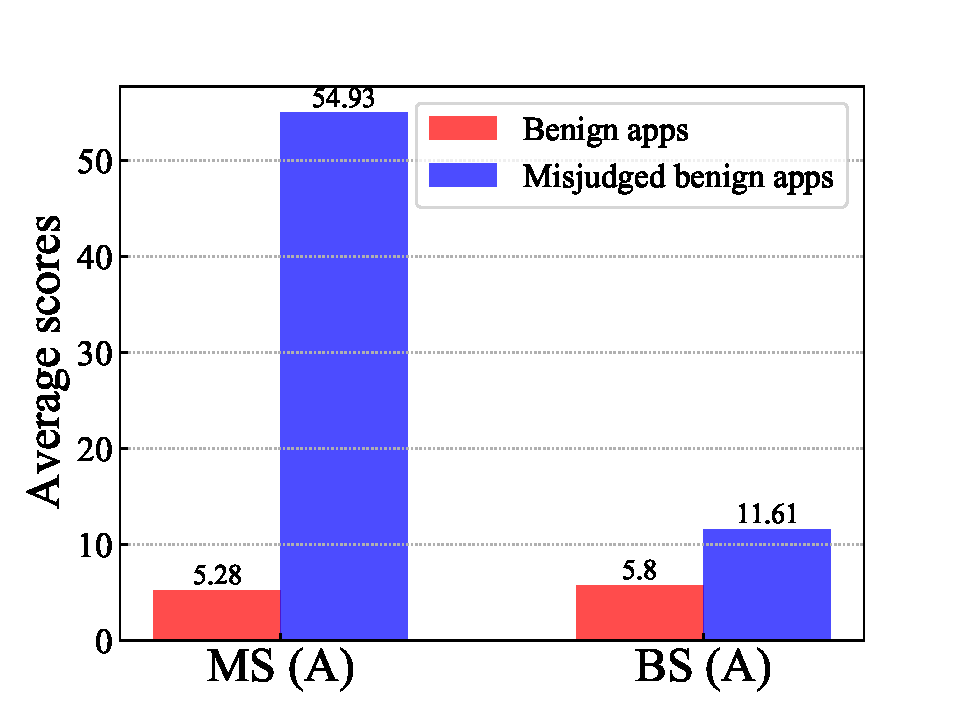
\includegraphics[scale=0.255]{./figures/bar_MS_(A)_BS_(A)_benign_apps.pdf}
  } 
  \subfigure[Custom permissions]{ %
    \label{fig:score_c_ben} 
    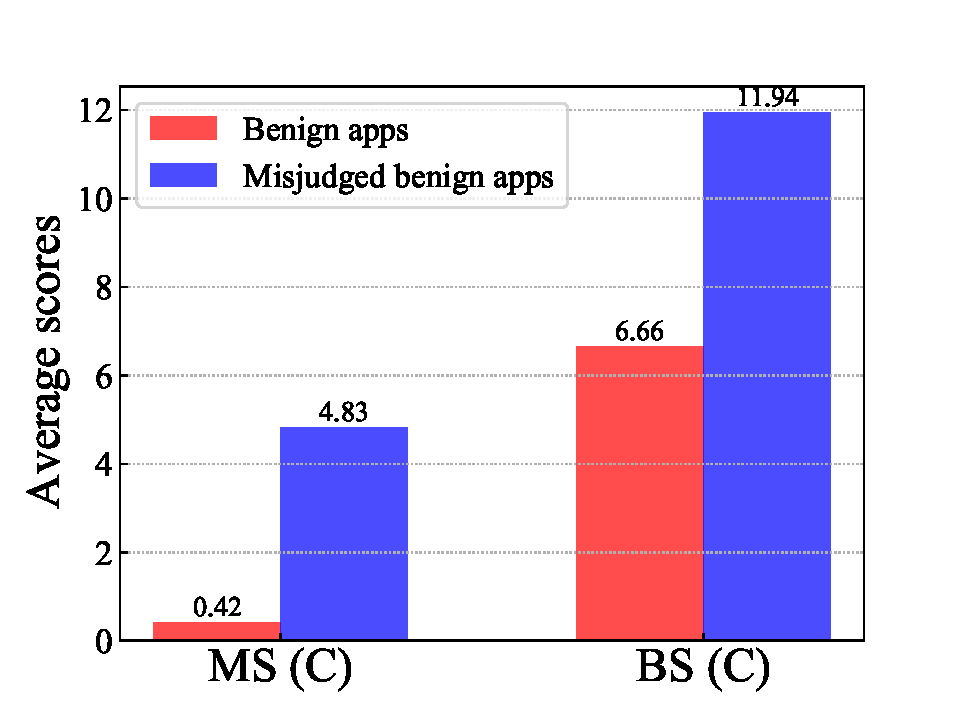
\includegraphics[scale=0.255]{./figures/bar_MS_(C)_BS_(C)_benign_apps.pdf}
  } 
  \subfigure[Dangerous permissions]{ %
    \label{fig:score_d_ben} 
    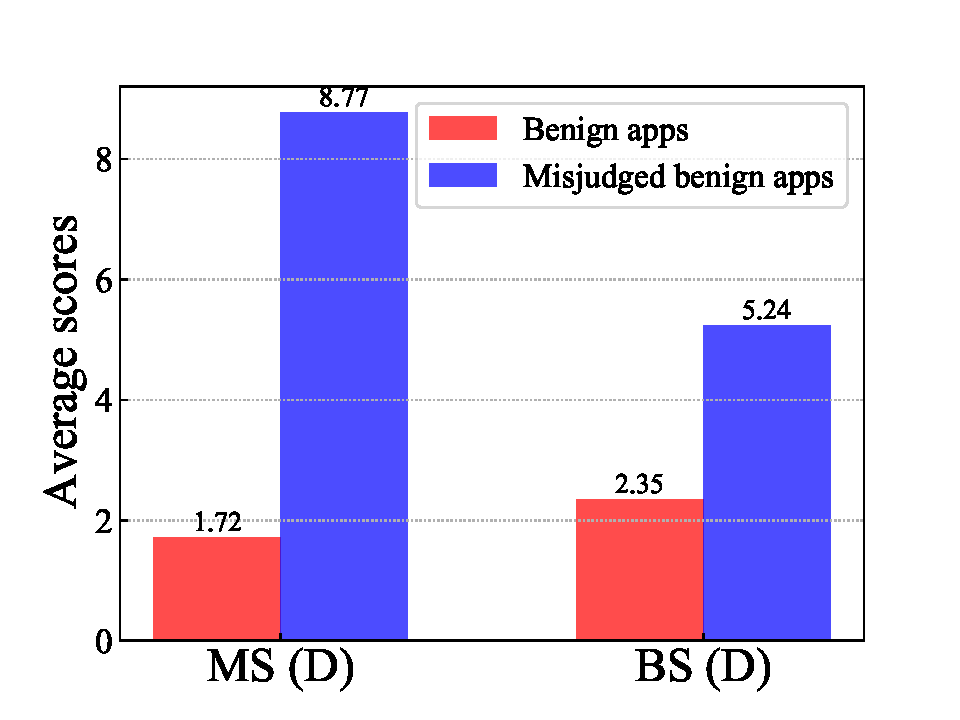
\includegraphics[scale=0.255]{./figures/bar_MS_(D)_BS_(D)_benign_apps.pdf}
  } 
  \subfigure[All permissions]{ %
    \label{fig:score_all_ben} 
    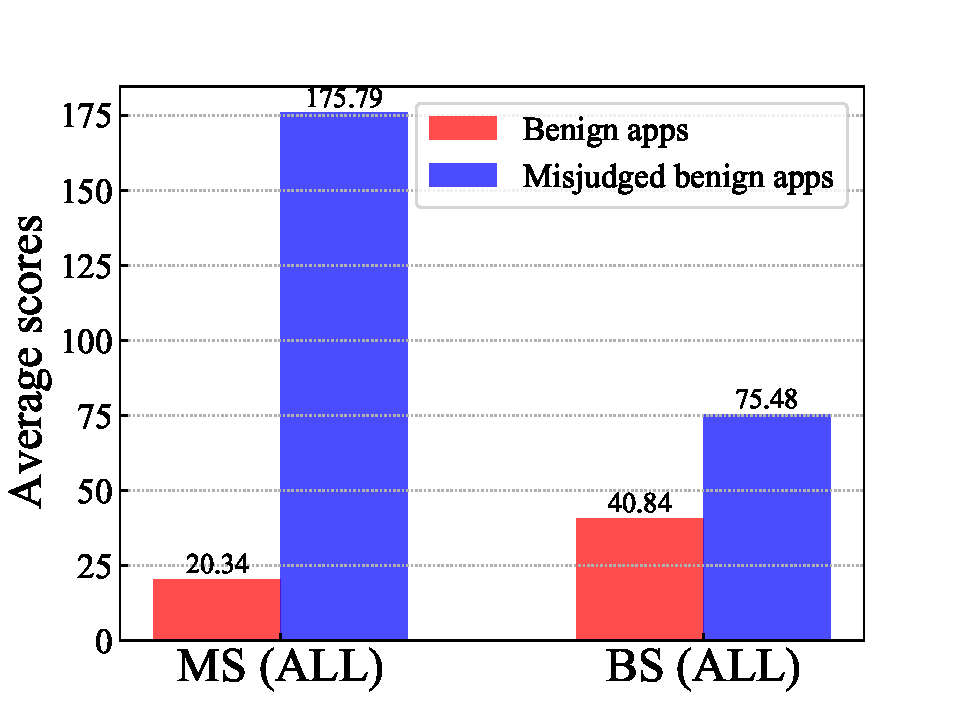
\includegraphics[scale=0.255]{./figures/bar_MS_(ALL)_BS_(ALL)_benign_apps.pdf}
  } 
  \caption{Average proposed scores of benign apps and misjudged ones.}
  \label{fig:score_ben}
\end{figure*}
\begin{figure*}[t]
  \centering
  \subfigure[Android permissions]{%
    \label{fig:android_p_dist_ben} 
    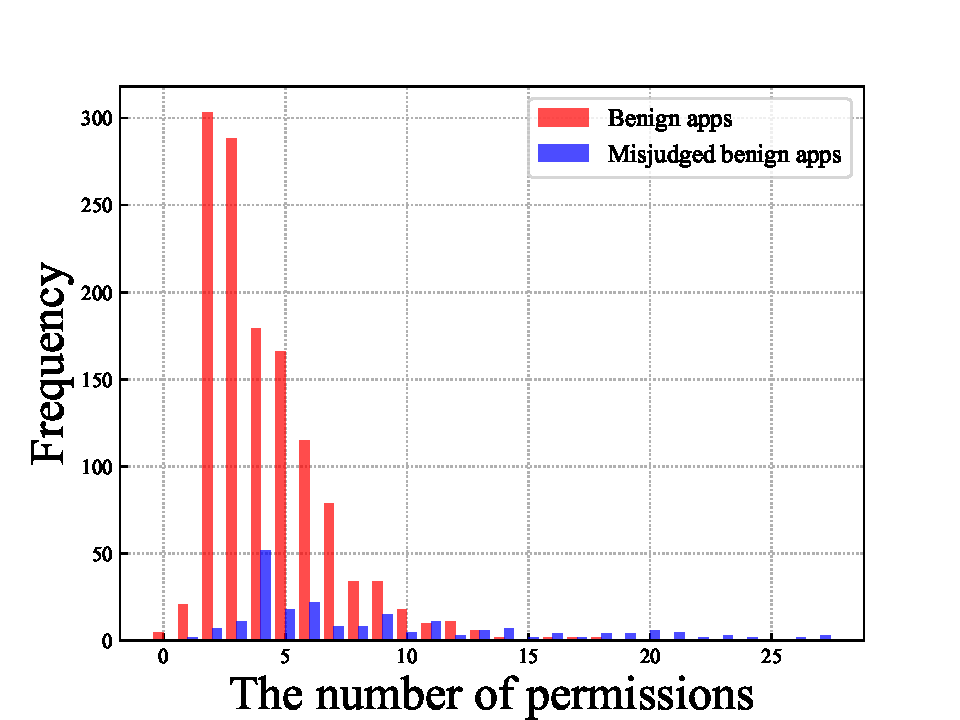
\includegraphics[scale=0.255]{./figures/benign_android_dist.pdf}
  } 
  \subfigure[Custom permissions]{ %
    \label{fig:custom_p_dist_ben} 
    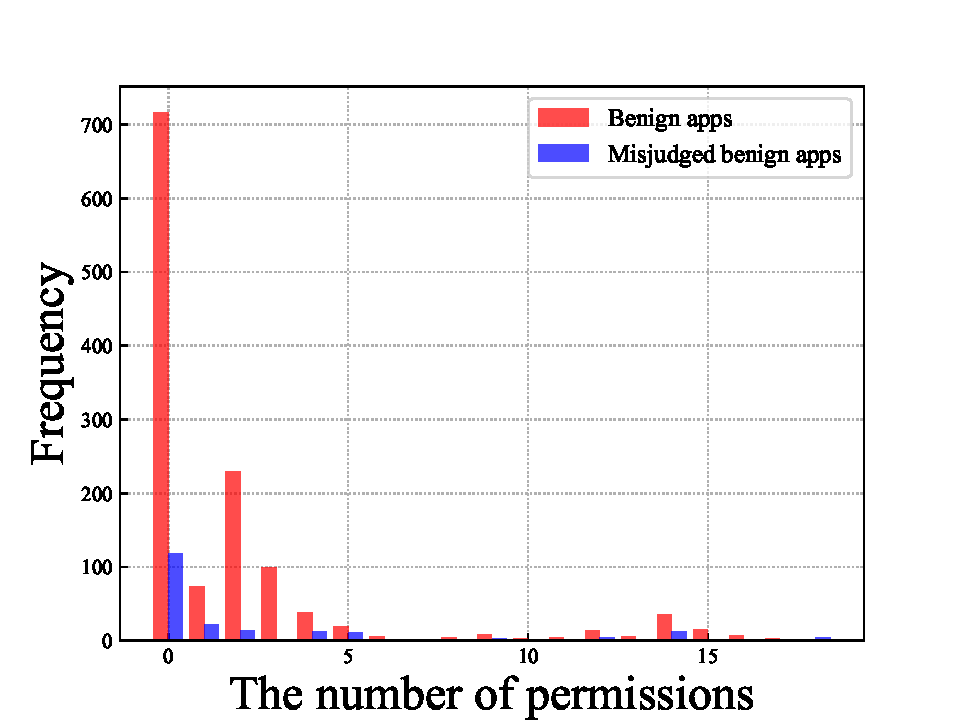
\includegraphics[scale=0.255]{./figures/benign_cumsum_dist.pdf}
  } 
  \subfigure[Dangerous permissions]{ %
    \label{fig:dangerous_p_dist_ben} 
    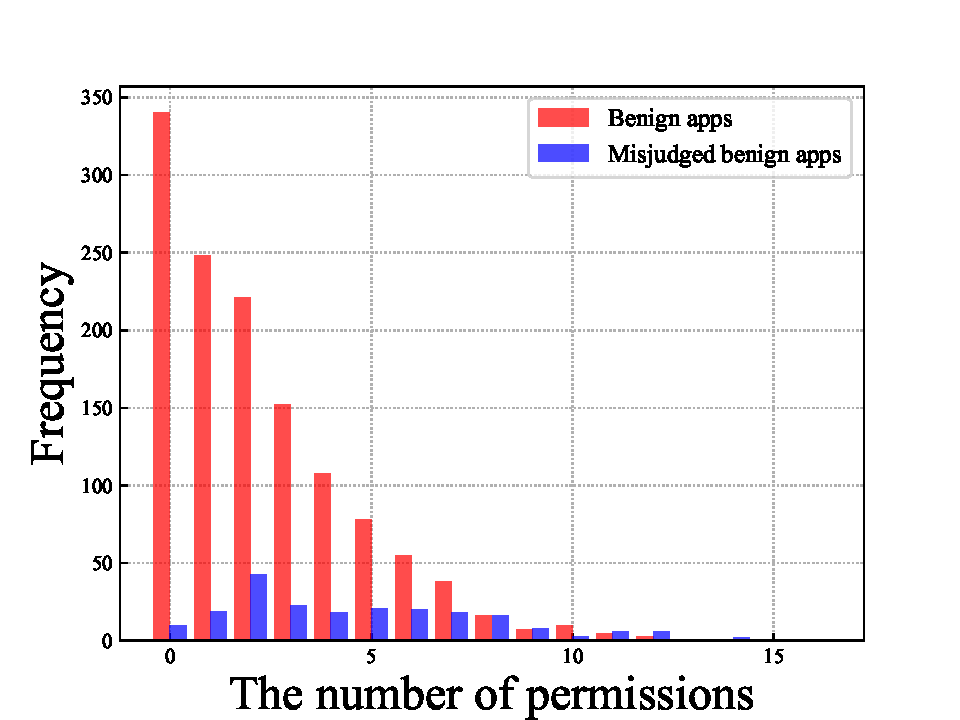
\includegraphics[scale=0.255]{./figures/benign_dangerous_dist.pdf}
  } 
  \subfigure[All permissions]{ %
    \label{fig:all_p_dist_ben} 
    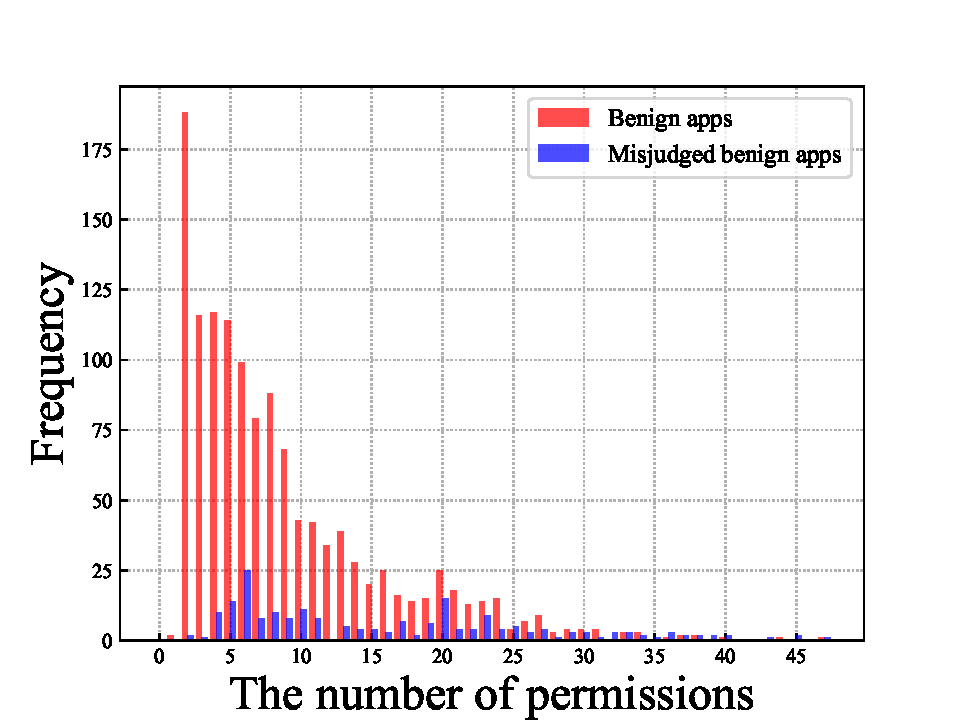
\includegraphics[scale=0.255]{./figures/benign_all_dist.pdf}
  } 
  \caption{Distribution of the number of permissions required by benign apps and misjudged ones.}
  \label{fig:permission_distribution_ben}
\end{figure*}
\subsubsection{Analysis for Misjudged Benign Apps} \label{subsec:analysis_mis_benign}
On the other hand, as shown in \myfigurename~\ref{fig:score_a_ben}, \myfigurename~\ref{fig:score_d_ben}, and \myfigurename~\ref{fig:score_all_ben}, magnitude correlation between MSs and BSs in misjudged benign apps (blue bars) are reversed compared with those in benign apps (red bars) except for MS (C) and BS (C) in \myfigurename~\ref{fig:score_c_ben}.
From this result, it turns out that CPs are less important than other permissions.
Furthermore, the differences between MSs and BSs in misjudged benign apps are large compared with those in benign apps.
Thus, these large differences causes misjudgement in the proposed scheme.
\myfigurename~\ref{fig:permission_distribution_ben} shows distribution of the number of permissions required by benign apps and misjudged ones.
As shown in \myfigurename~\ref{fig:android_p_dist_ben}, \myfigurename~\ref{fig:dangerous_p_dist_ben} and \myfigurename~\ref{fig:all_p_dist_ben}, misjudged benign apps is liable to require more permissions. 
In this case, CRs of permission pairs in such benign apps are similar to the ones in malware because CRs get small.
Hence, the proposed scheme regards the benign apps as malware by mistake when many permissions are required by benign apps.
In order to prevent this types of misjudgement, it is important that developers of benign apps should avoid requiring unnecessary permissions.
On the other hand, attackers have no choice but to inject unnecessary permission so as to conceal malicious evidence in permissions.
Considering this fact, misjudgement by our scheme can be prevented by obeying the right manner of development in terms of permissions.  

Meanwhile, the proposed scheme also failed in judging benign apps that require fewer permissions whereas the tendency of the CR of permission pairs is relatively similar to the benign one.
To reveal the reason, we investigated such benign apps.
After our investigation, we discovered that a benign app requires six permissions including three DPs, namely SEND\_SMS (SSMS), READ\_SMS (RSMS), and RECEIVE\_SMS (RECSMS).
MS (D) and BS (D) are 2.03 and 0.0, respectively.
In addition to these DPs, this benign app also has INTERNET.
By combining this permission and the above DPs, this benign app is potentially capable to conduct malicious operations.
% INT:SSMS$B$H$+$N%Z%"$NN`;wEY$r0l$D8+$;$k!)!)(B
In fact, in terms of the pair INT:SSMS, similarities, $\SMAL$ and $\SBEN$ are 0.9349 and 0.9336, respectively, which means that this benign app is more similar to malware.
As for other pairs such as INT:RSMS and INT:RECSMS, we found that $\SMAL$ is larger than $\SBEN$.
As a result, MS (ALL) and BS (ALL) are 11.2 and 2.83, respectively.
% Therefore, these types of benign apps can be misjudged as malware.
To cope with this misjudgement, using other features such as API calls and ICC is needed.
  % MS (A)     BS (A)    MS (C)     BS (C)     MS (D)     BS (D)    MS (ALL)    BS (ALL)
% 0.000000    0.061420    0.000000    0.000000    2.032634   0.000000    11.220711     2.834962

% $BIQEY$N9b$$$b$N$rMW5a$7$F$bN`;wEY$K:9$,=P$k$+$iH=CG:`NA$r$"$?$($k$3$H$,$G$-$k!#(B

% \subsubsection{False Positive Analysis}

% $B8m8!CN$7$?NI@-$@$1$NFCD'NL$NJ?6QCM$H$+$NHf3S$r?^$G<($9!#(B
% $BB?$/$N%Q!<%_%C%7%g%s$rMW5a$9$kNI@-%"%W%j$K$OBP1~$G$-$J$$!#(B
% $B$=$N:]$O!"B>$N4QE@$b9MN8$9$kI,MW$,$"$k$G$"$m$&!#(B
% $B$7$+$7!"3+H/<T$,ITI,MW$K%Q!<%_%C%7%g%s$rMW5a$9$k$3$H$r$5$1$l$P!"$3$N8m8!CN$O5/$-$J$$!#(B
% $B0lJ}$G0-@-$O!"NI@-$K;w$;$k$?$a$KITI,MW$J$b$N$rMW5a$7$F$*$j!"Ds0FJ}<0$rHr$1$k$?$a$K!"ITI,MW$J$b$N$rF~$l$J$1$l$P!"5U$KC1=c$K=>Mh$NJ}<0$G8!CN$5$l$F$7$^$&$?$a!"F~$l$6$k$rF@$J$$!#(B
% $BNI@-%"%W%j$N3+H/<T$,!"ITI,MW$KB?$/$N8"8B$rMW5a$9$k$3$H$O!"8=<B$K$O5/$3$j$K$/$$$H9M$($i$l!"==J,KI$0$3$H$,$G$-$k!#(B



\section{Limitation} \label{sec:limitation}
Our scheme can satisfy requirements for practical use.
However, there exist some limitations even in the proposed scheme.
% 1. $B%Q!<%_%C%7%g%s$r@EE*$KMW5a$7$J$$$h$&$J0-@-%"%W%j$K$OBP1~$G$-$J$$!#(B
The first one is that the proposed scheme cannot deal with malware samples that statically require fewer permissions, as explained in Section~\ref{subsec:analysis} 2).
% The reason for this is that permissions may be dynamically required.
This limitation is common to all the permission based schemes that utilize static analysis \cite{li2018significant, liang2014permission, liu2014two, arora2019permpair}.
In order to address this limitation, extracting dynamic permissions \cite{mahindru2017dynamic} is promising.
We plan to devise a new scheme that calculates the CR from pairs of permissions including dynamic ones.
However, in order to obtain dynamic permissions, it is necessary to run each app in a device or an emulator, which causes runtime overhead.
Since dynamic analysis based schemes can also capture more useful features such as network traffic and API calls, the feature fusion may be more useful.
In light of such facts and the compatibility of our low-dimensional features, combining our features and other features can be promising for detecting the above malware.
% 2. $B%G!<%?%Y!<%9$rJ]4I$9$kI,MW$,$"$k$?$a!"J];}$9$k%G!<%??t$,B?$/$J$k2DG=@-$,$"$k!#(B

Furthermore, as mentioned in Section~\ref{subsec:analysis} 4), our scheme cannot correctly judge benign apps that require fewer permissions including DPs.
Such benign apps might actually need to use DPs for benign purposes.
It is difficult to justify the truth on the basis of information about permissions.
Thus, we concluded that such benign apps should be treated by using other feature based schemes.
% To overcome the limitation, in the future, we plan to devise more functional schemes with other feature.

At this stage, our scheme utilizes all permission pairs required by apps.
As a result, detection performance of the proposed scheme is slightly inferior to BVBS with pairs of more than 80 permissions.
In order to ameliorate the performance, we might have to select useful pairs from all pairs.
It is possible that using only pairs whose variance of the CR is small is helpful in improving detection performance.
We will work on this task as future work.
% $BA4$F$N%Z%"$r9MN8$G$-$k$,!"8!CNN($,<c43Dc$$$N$G!"M-MQ$J%Z%"$NA*BrJ}$r9M$($k!#(B
% $BA4$F$N%Z%"$r9MN8$7$F$b!"8zN(E*$J$N$G!"$5$i$K8zN(E($K$J$k2DG=@-$b$"$k$?$a!"(BFW$B$K;D$9$h!#(B

% $B$7$+$7!"9MN8$9$Y$-%Z%"$J$I$rA*Br$9$kJ}K!$r9M$($k$3$H$G!"2r7h$G$-$k$+$b$7$l$J$$!#(B
% 3. $B$^$?!"5!3#3X=,%Y!<%9$J$N$G!"(BAdversarial Example$B$J$I$N967b$N1F6A$b7|G0$5$l$k!#(B
% $B$7$+$7!"(B1$B$D$N%Q!<%_%C%7%g%s$rF~$l$k$4$H$KJ#?t$N%Z%"$,$G$-$k$?$a!"Fq$7$$$+$b$7$l$J$$!#(B
% 4.$B$^$?!"6&KE967b$J$I$K$OBP1~$G$-$J$$2DG=@-$,$"$k!#(B
% $B$7$+$7!"(BICC$B$J$I$NJ}<0$rAH$_9g$o$;$l$P!"$=$3$OJd$($k!#(B

\section{Conclusion and future work} \label{sec:conclusion}
In this paper, we have proposed Android malware detection scheme using the CR of permission pairs.  
We focus on the fact that the CR tends to be small in malware because of unnecessary permissions.
To leverage the CR for malware detection, we constructed databases regarding the CR.
% For each class (benign apps and malware), four CR based databases are constructed from four aspects in terms of permissions, namely Android Permission (AP), Custom Permission (CP), Dangerous Permission (DP), and all permissions.
% In other words, the eight databases are prepared in total.  
For each app, we calculated eight similarity scores on the basis of the prepared databases.
% For each app, we calculate a similarity score for benign apps and one for malware on the basis of the databases.
% By doing this, even if malware requires unnecessary permissions, the effective features can be obtained from a new aspect.
Finally, our scores were fed into machine learning (ML) based classifiers for detection.
% The proposed scheme utilizes just eight-dimensional features, it can reduce training time and compatibility with other features, which means our scheme is efficient. 
% Our features are just eight-dimensional.
% Our scores are easy to be understood because information about required permission pairs can be expressed as eight simple scores.
% Thus, since understandable information are provided for human, the proposed scheme also meets ``Intelligibility'', which is suitable for practical use.
By using real datasets, our evaluation results show that the proposed scheme can detect malware with up to 97.3\% accuracy.
% In terms of recent malware samples, our scheme can detect them with the high accuracy.
% convert information about permission pairs into just eight-dimensional features with maintaining comparable detection accuracy compared with a conventional scheme.
% Compared with a existing method, our scheme can reduce training time by about 91\% with maintaining comparable detection accuracy.
Compared with BVBS, our scheme can reduce the feature dimensions by about 99\% with maintaining comparable detection accuracy on recent datasets.
Because of this, the proposed scheme is compatible with other features in ML based schemes.
Furthermore, our features can quantitatively offer clear information that what types of permission pairs dictate detection results.
Thus, our scheme is more suitable for practical use.
However, our scheme has the limitations.
To address them, our future work will focus on devising a new scheme that calculates the CR from pairs of permissions including dynamic ones.
% our future work will focus on devising more functional schemes that combine CR based scores with other features.
Besides, in order to improve detection performance, we plan to select useful pairs by using some techniques such as clustering CRs with their variance in future.

\bibliographystyle{IEEEtran}% bib style
\bibliography{IEEE_ref}

\begin{IEEEbiography}[{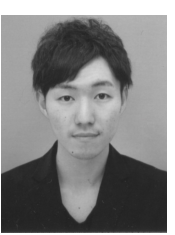
\includegraphics[width=1in,height=1.25in,clip,keepaspectratio]{./figures/kato.pdf}}]{Hiroya Kato} was born in Gunma, Japan in 1994. He received his B.E. and M.E. degrees from Keio University, in 2017 and 2019, respectively, where he is currently pursuing the Ph.D. degree. His research interest is security \& privacy for IoT. He is a member of IEICE.
\end{IEEEbiography} 

\begin{IEEEbiography}[{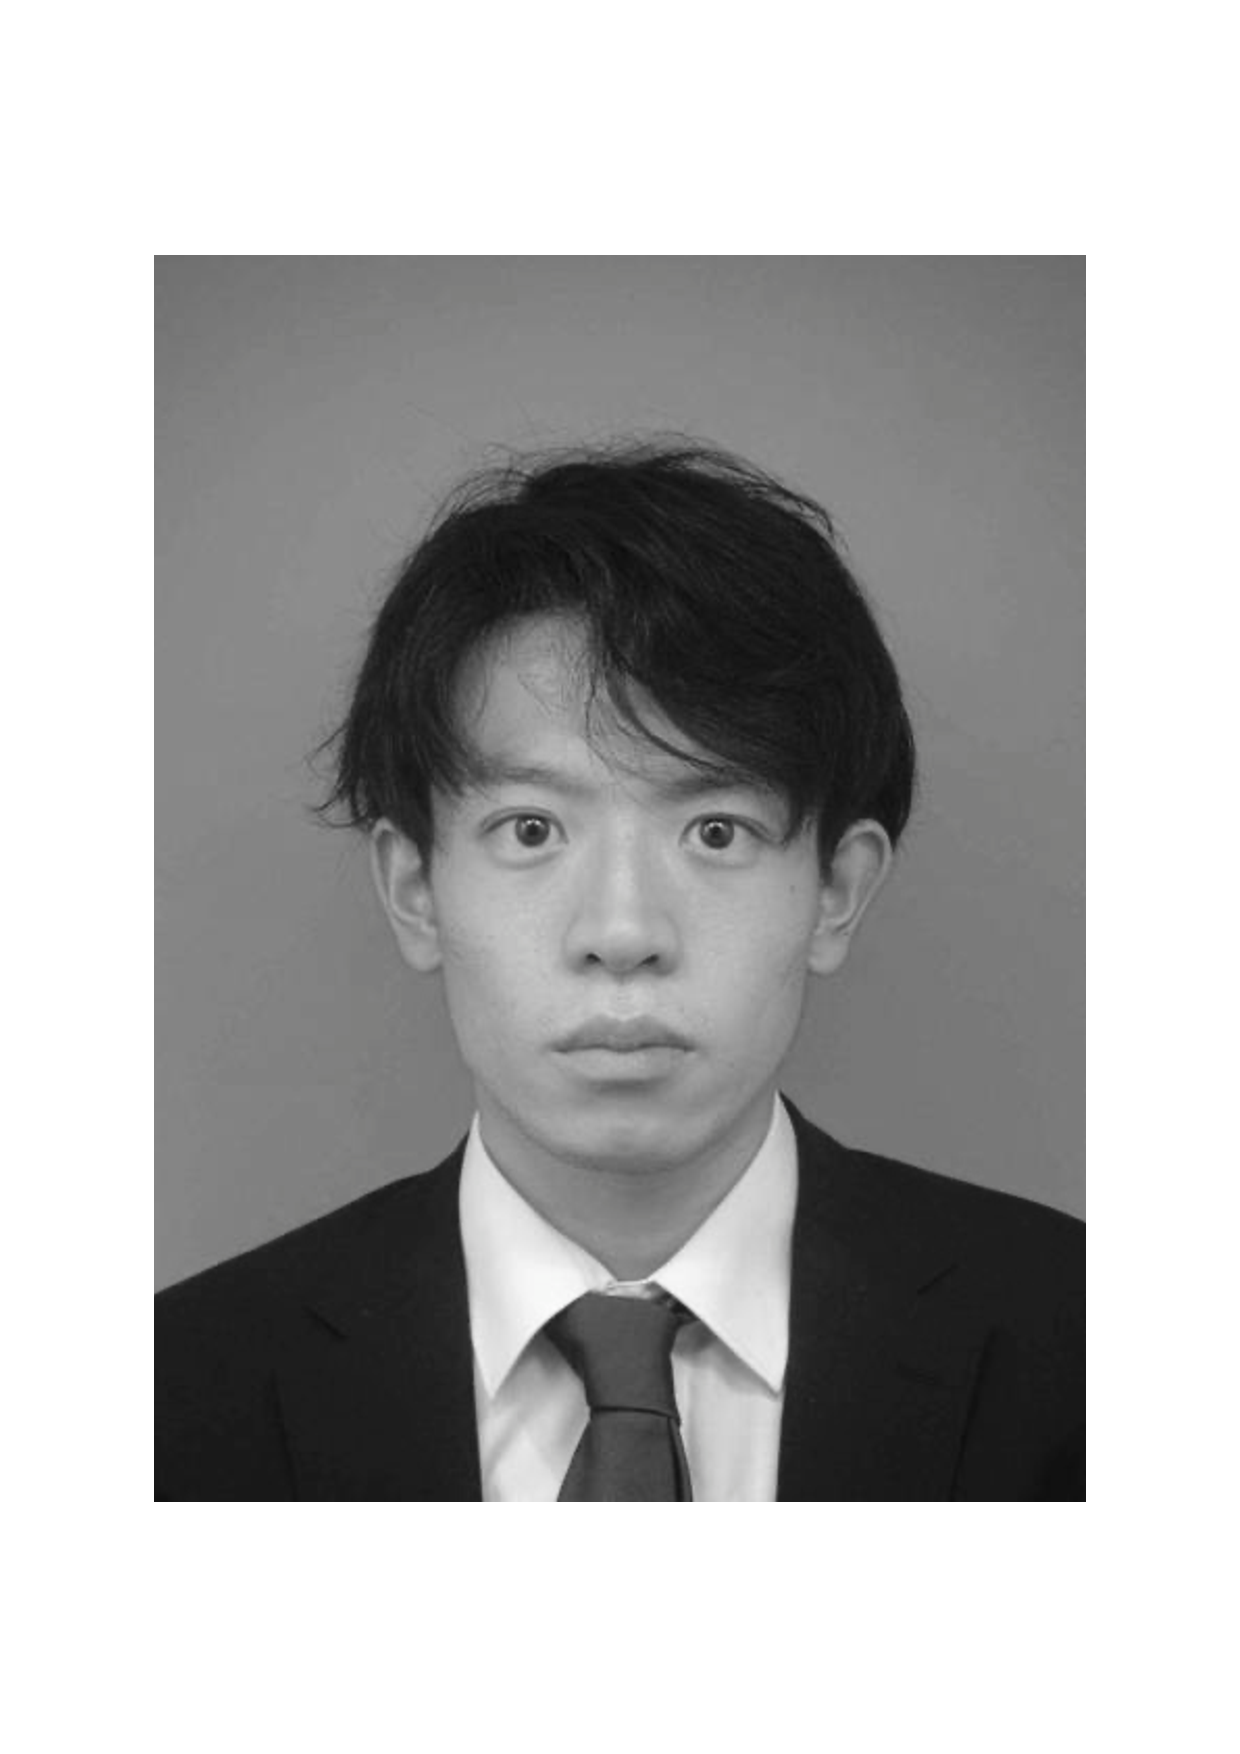
\includegraphics[width=1in,height=1.25in,clip,keepaspectratio]{./figures/sasak.pdf}}]{Takahiro Sasaki} was born in Saitama, Japan in 1995. He received his B.E. degrees from Keio University in 2021. His research interest is security \& privacy for IoT.
\end{IEEEbiography}

\begin{IEEEbiography}[{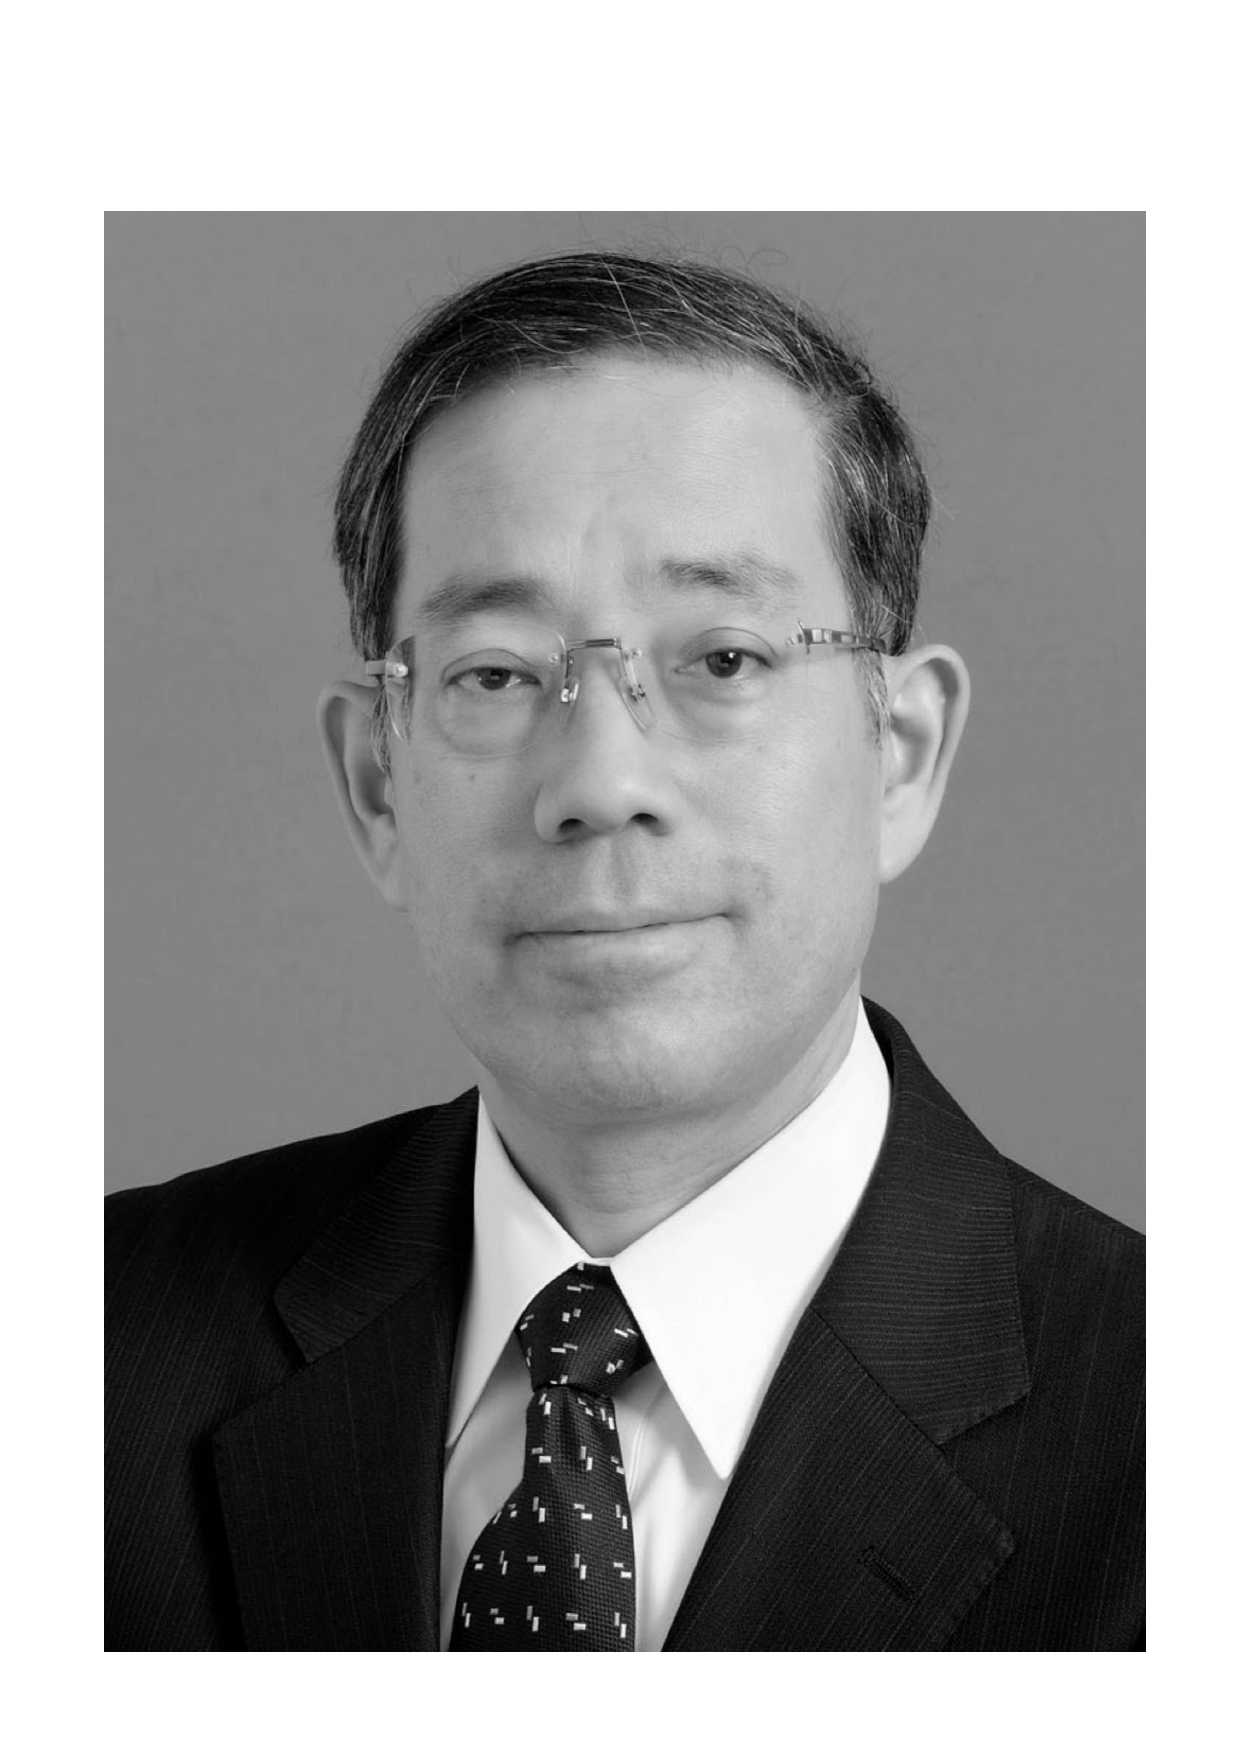
\includegraphics[width=1in,height=1.25in,clip,keepaspectratio]{./figures/sasas.pdf}}]{Iwao Sasase} was born in Osaka, Japan in 1956. He received the B.E., M.E., and D.Eng. degrees in Electrical Engineering from Keio University, Yokohama, Japan, in 1979, 1981 and 1984, respectively. From 1984 to 1986, he was a Post Doctoral Fellow and Lecturer of Electrical Engineering at the University of Ottawa,ON, Canada. He is currently a Professor of Information and Computer Science at Keio University, Yokohama, Japan. His research interests include modulation and coding, broadband mobile and  wireless communications, optical communications, communication networks and information theory. He has authored more than 301 journal papers and 446 international conference papers. He granted 48 Ph.D. degrees to his students in the above field. Dr. Sasase received the 1984 IEEE Communications Society (ComSoc) Student Paper Award (Region 10), 1986 Inoue Memorial Young Engineer Award, 1988 Hiroshi Ando Memorial Young EngineerAward, 1988 Shinohara MemorialYoung EngineerAward, 1996 Institute of Electronics, Information, and Communication Engineers (IEICE) of Japan Switching System Technical Group Best Paper Award, and WPMC2008 Best Paper Award. He is now serving as a Vice-President of IEICE. He served as President of the IEICE Communications Society (2012-2014). He was Board of Governors Member-at-Large (2010-2012), Japan Chapter Chair (2011-2012), Director of the Asia Pacific Region (2004-2005), Chair of the Satellite and Space Communications Technical Committee (2000-2002) of IEEE ComSoc., Vice President of the Communications Society (2004-2006), Chair of the Network System Technical Committee (2004-2006), Chair of the Communication System Technical Committee (2002-2004) of the IEICE Communications Society, Director of the Society of Information Theory and Its Applications in Japan (2001-2002). He is Fellow of IEICE, and Senior Member of IEEE, Member of the Information Processing Society of Japan.
\end{IEEEbiography}

\endgroup
\EOD
\end{document}
